% ============================================================
% Beamer — ISLP Lecture Series — IMPROVED EDITION
% Chapter 12: Unsupervised Learning
% ============================================================
\documentclass[aspectratio=169,11pt]{beamer}
\usepackage[utf8]{inputenc}\usepackage[T1]{fontenc}\usepackage[english]{babel}
\usepackage{graphicx}\usepackage{booktabs}\usepackage{amsmath,amssymb,amsfonts}
\usepackage{mathtools}\usepackage{hyperref}\usepackage{xcolor}\usepackage{colortbl}
\usepackage{verbatim}\usepackage{alltt}
\usepackage{tikz}\usetikzlibrary{calc,arrows.meta,positioning,shapes}
\usepackage{tcolorbox}\tcbuselibrary{skins}

\usetheme{Madrid}\usecolortheme{default}
\setbeamertemplate{navigation symbols}{}
\setbeamertemplate{footline}[frame number]
\setbeamertemplate{blocks}[rounded][shadow=false]
\setbeamertemplate{headline}{%
  \leavevmode\hbox{%
    \begin{beamercolorbox}[wd=\paperwidth,ht=2.2ex,dp=0.9ex]{section in head/foot}%
      {\fontsize{4.6}{5.2}\selectfont%
       \insertsectionnavigationhorizontal{\paperwidth}{}{\hskip0pt plus1filll}}%
    \end{beamercolorbox}}%
}
\setbeamerfont{section in head/foot}{size=\tiny}
\setbeamerfont{palette primary}{size=\tiny}
\setbeamerfont{palette tertiary}{size=\tiny}
\setbeamerfont{section in toc}{size=\footnotesize}

\usepackage{listings}
\definecolor{pyKw}{RGB}{0,0,180}\definecolor{pyStr}{RGB}{20,120,40}
\definecolor{pyCom}{RGB}{120,120,120}\definecolor{accent}{RGB}{38,70,140}
\lstdefinestyle{Pystyle}{language=Python,basicstyle=\ttfamily\footnotesize,
  keywordstyle=\color{pyKw}\bfseries,commentstyle=\color{pyCom}\itshape,
  stringstyle=\color{pyStr},showstringspaces=false,upquote=true,
  columns=fullflexible,breaklines=true,literate={~}{{$\sim$}}1}
\lstset{style=Pystyle}

\AtBeginSection[]{\begin{frame}{Outline}\footnotesize
  \tableofcontents[currentsection,sectionstyle=show/shaded,subsectionstyle=show/show/hide]
\end{frame}}

\newcommand{\islpsource}[1]{%
  \vfill\hfill{\tiny\itshape\color{gray}Source: #1 \textemdash{} ISLP, James et al.\ (2023).}\par
}

\newtcolorbox{takeaway}[1][Takeaway]{enhanced,colback=green!4,colframe=green!50!black,
  boxrule=0pt,leftrule=2.5pt,arc=2pt,fonttitle=\bfseries,title=#1,
  left=2mm,right=2mm,top=1mm,bottom=1mm}
\newtcolorbox{numexample}[1][Worked example]{enhanced,colback=orange!4,colframe=orange!70!black,
  boxrule=0pt,leftrule=2.5pt,arc=2pt,fonttitle=\bfseries,title=#1,
  left=2mm,right=2mm,top=1mm,bottom=1mm}
\newtcolorbox{readme}[1][How to read this]{enhanced,colback=blue!4,colframe=accent,
  boxrule=0pt,leftrule=2.5pt,arc=2pt,fonttitle=\bfseries,title=#1,
  left=2mm,right=2mm,top=1mm,bottom=1mm}

\title{Quantitative Research Methods}
\subtitle{Chapter 12: Unsupervised Learning}
\author{Prof.\ Dr.\ Christoph Weisser}
\date{}\graphicspath{{images/}}

\newtcolorbox{exercise}[1][Exercise]{enhanced, fontupper=\footnotesize, colback=purple!4, colframe=purple!55!black, boxrule=0pt, leftrule=2.5pt, arc=2pt, fonttitle=\bfseries, title=#1, left=2mm, right=2mm, top=1mm, bottom=1mm}
\newtcolorbox{solutionbox}[1][Solution]{enhanced, fontupper=\footnotesize, colback=teal!5, colframe=teal!55!black, boxrule=0pt, leftrule=2.5pt, arc=2pt, fonttitle=\bfseries, title=#1, left=2mm, right=2mm, top=1mm, bottom=1mm}
\newtcolorbox{longexercise}[1][Extended exercise (15 min)]{enhanced, fontupper=\footnotesize, colback=violet!6, colframe=violet!55!black, boxrule=0pt, leftrule=3pt, arc=2pt, fonttitle=\bfseries, title=#1, left=2mm, right=2mm, top=1mm, bottom=1mm}

% Reclaim ~2pt of body height (custom nav headline makes full slides tip over by ~1.83pt)
\addtobeamertemplate{frametitle}{}{\vspace{-2pt}}

\newtcolorbox{labnote}[1][Run this live in the lab notebook]{enhanced, fontupper=\footnotesize, colback=cyan!7, colframe=cyan!45!black, boxrule=0pt, leftrule=3pt, arc=2pt, fonttitle=\bfseries, title=#1, left=2mm, right=2mm, top=1mm, bottom=1mm}

% Industry application callout box --- slate grey, for real business/industry use
\definecolor{industryC}{RGB}{88,98,116}
\newtcolorbox{industry}[1][In industry]{enhanced, fontupper=\footnotesize, colback=industryC!7, colframe=industryC, boxrule=0pt, leftrule=3pt, arc=2pt, fonttitle=\bfseries, title={In industry --- #1}, left=2mm, right=2mm, top=1mm, bottom=1mm}

% Common-mistake callout --- crimson, for the error to pre-empt
\newtcolorbox{mistake}[1][Common mistake]{enhanced, fontupper=\footnotesize, colback=red!4, colframe=red!60!black, boxrule=0pt, leftrule=3pt, arc=2pt, fonttitle=\bfseries, title=#1, left=2mm, right=2mm, top=1mm, bottom=1mm}

\begin{document}
\begin{frame}[plain]\titlepage\end{frame}

\begin{frame}{The course at a glance}
  \vspace{-1.5mm}
  \begin{center}
  \scriptsize
  \setlength{\tabcolsep}{5pt}
  \renewcommand{\arraystretch}{1.30}
  \begin{tabular}{@{\hspace{2pt}}l >{\raggedright\arraybackslash}p{0.66\textwidth}@{\hspace{2pt}}}
    \toprule
    \textbf{Chapter} & \textbf{Topic} \\
    \midrule
     {\color{accent}Ch.\ 1} & Introduction \\
    \rowcolor{black!3} {\color{accent}Ch.\ 2} & Statistical learning\,{\color{black!45}--- accuracy, bias--variance, Bayes classifier, KNN} \\
     {\color{accent}Ch.\ 3} & Linear regression\,{\color{black!45}--- estimation, inference, diagnostics} \\
    \rowcolor{black!3} {\color{accent}Ch.\ 4} & Classification\,{\color{black!45}--- logistic regression, confusion matrix, ROC} \\
     {\color{accent}Ch.\ 5} & Resampling\,{\color{black!45}--- validation, CV, bootstrap} \\
    \rowcolor{black!3} {\color{accent}Ch.\ 6} & Model selection and regularisation\,{\color{black!45}--- ridge, lasso} \\
     {\color{accent}Ch.\ 7} & Moving beyond linearity\,{\color{black!45}--- splines, GAMs} \\
    \rowcolor{black!3} {\color{accent}Ch.\ 8} & Tree-based methods\,{\color{black!45}--- trees, forests, boosting} \\
     {\color{accent}Ch.\ 10} & Deep learning\,{\color{black!45}--- MLPs, CNNs, training} \\
    \rowcolor{accent!18} \textbf{Ch.\ 12} & \textbf{Unsupervised learning}\,{\color{accent!75!black}--- PCA, clustering} \\
    \bottomrule
  \end{tabular}
  \end{center}
  \vspace{1mm}
  {\scriptsize Ten chapter decks of 180 minutes each, after a taught precourse session; Chapters 2, 3 and 4 run over two sessions apiece. Today's chapter is highlighted. Short exercises every $\sim$20 min; extended exercises every $\sim$45 min; each chapter has a companion lab notebook.\par\medskip Support vector machines (Ch.\ 9), survival analysis (Ch.\ 11) and multiple testing (Ch.\ 13) are optional self-study modules in \texttt{Chapters/Advanced/}.}
\end{frame}

\begin{frame}{Contents}\small\tableofcontents[hideallsubsections]
  \vfill
  {\tiny Optional and advanced material is collected in the \textbf{appendix} at the end of the deck.}
\end{frame}

\begin{frame}{Notation in this chapter}
  \footnotesize
  \begin{center}
  \begin{tabular}{@{}ll@{}}
    \toprule
    \textbf{Symbol} & \textbf{Meaning} \\
    \midrule
    $n$, $p$ & number of observations; number of features (no response $Y$ anywhere) \\
    $x_{ij}$ & value of feature $j$ for observation $i$, always \emph{centred} (mean $0$) \\
    $\phi_{jm}$ & loading of feature $j$ on the $m$-th principal component \\
    $\phi_m=(\phi_{1m},\dots,\phi_{pm})^\top$ & the $m$-th loading vector, normalised to $\|\phi_m\|=1$ \\
    $z_{im}$ & score of observation $i$ on component $m$; $z_{im}=\sum_j \phi_{jm}x_{ij}$ \\
    $\lambda_m$ & variance of the $m$-th score vector (the $m$-th eigenvalue) \\
    $\mathrm{PVE}_m$ & proportion of variance explained by component $m$ \\
    $M$ & number of components retained \\
    $K$ & number of clusters \\
    $C_1,\dots,C_K$ & the clusters: a partition of $\{1,\dots,n\}$; $|C_k|$ is the size of $C_k$ \\
    $\bar x_{kj}$ & mean of feature $j$ inside cluster $C_k$ (the $j$-th centroid coordinate) \\
    $W(C_k)$ & within-cluster variation of $C_k$; \ $W=\sum_k W(C_k)$ \\
    $d(i,i')$ & dissimilarity between observations $i$ and $i'$ \\
    $d(A,B)$ & linkage: dissimilarity between two \emph{groups} $A$ and $B$ \\
    $r_{ii'}$ & correlation between the feature profiles of observations $i$ and $i'$ \\
    $s_i$ & silhouette width of observation $i$ \\
    \bottomrule
  \end{tabular}
  \end{center}
\end{frame}

\begin{frame}{Sources and references}
  \begin{block}{Primary textbook}
    James, G., Witten, D., Hastie, T., Tibshirani, R., \& Taylor, J.\ (2023).
    \emph{An Introduction to Statistical Learning, with Applications in
    Python.} Springer.
  \end{block}
  \begin{readme}[{{Data used in this chapter}}]
    \texttt{USArrests} --- four crime and urbanisation measures for the $50$ US states;
    the textbook's PCA example. \texttt{Ch12Ex13} --- $1000$ genes measured on
    $40$ tissue samples ($20$ healthy, $20$ diseased), the textbook's
    high-dimensional clustering exercise.
  \end{readme}
\end{frame}

\begin{frame}{Learning objectives}
  By the end of this chapter you will be able to:
  \begin{itemize}
    \item \textbf{Explain} why unsupervised learning has no test error, and what
          that costs you.
    \item \textbf{Apply} principal component analysis, and read loadings, scores,
          a biplot and a scree plot.
    \item \textbf{Decide} whether to standardise the features --- and show what
          happens if you do not.
    \item \textbf{Run} $K$-means, and defend the result against its
          local-optimum problem.
    \item \textbf{Build} and cut a dendrogram, choosing a linkage and a
          dissimilarity measure on purpose.
    \item \textbf{Avoid} reporting clusters found in noise as if they were
          findings.
  \end{itemize}
\end{frame}

\begin{frame}{Roadmap of this chapter}
  \begin{takeaway}[{{Structure without a supervisor}}]
    \begin{enumerate}
      \item The hard part: no response, so \emph{no test error to validate against}.
      \item Principal component analysis: fewer variables, honestly reported.
      \item $K$-means: partition into $K$ groups, and the local-optimum trap.
      \item Hierarchical clustering: dendrograms, linkage, dissimilarity.
      \item Practice: scaling, outliers, clusters in pure noise, honest reporting.
    \end{enumerate}
  \end{takeaway}
\end{frame}

\begin{frame}{Where this chapter is used in industry}
  \scriptsize
  \begin{center}
  \begin{tabular}{@{}p{2.6cm}p{5.2cm}p{4.6cm}@{}}
    \toprule
    \textbf{Sector} & \textbf{Concrete application} & \textbf{Which decision it drives} \\
    \midrule
    Retail, banking & Customer segmentation from transaction and tenure features &
      Which segment gets which offer and service level \\
    Genomics, pharma & Clustering tumour samples by expression profile &
      Which subtype hypothesis goes into the next study \\
    Manufacturing & PCA on hundreds of correlated sensor channels &
      Which few indices the control room actually watches \\
    Finance & PCA of a yield curve: level, slope, curvature &
      How much interest-rate risk the book is carrying \\
    Marketing & Clustering of survey and behavioural data into personas &
      Which creatives and channels are built \\
    Insurance & Grouping claims by narrative and cost pattern &
      Which cases are routed to specialist handlers \\
    \bottomrule
  \end{tabular}
  \end{center}
  \begin{industry}[{{The common thread}}]
    In every row the output is a \textbf{hypothesis}, not a measurement. A segmentation is
    useful when the business acts on it and the action pays off --- that is the only
    validation available, and it arrives months later.
  \end{industry}
\end{frame}

\begin{frame}{Industry case in depth: a retail bank re-segments its customers}
  \footnotesize
  \begin{industry}[{{The task and the data}}]
    A bank wants a new customer segmentation from $\sim$$40$ features: balances, card
    spend, tenure, channel use, product holdings. There is no ``true segment'' column
    anywhere. The analytics team standardises the features, runs PCA to $8$ components
    ($\sim$$80\%$ of variance), then $K$-means at several $K$ with \texttt{n\_init=50}.
  \end{industry}
  \begin{readme}[{{What is decided, and by whom}}]
    The team proposes $K=6$ because $K=8$ produced two segments the relationship managers
    could not tell apart. Marketing, risk and the segment owners sign off. Nobody can
    compute an error rate: the segmentation is validated by a \textbf{live campaign} --- two
    segments get a tailored offer, two matched control groups do not, and the uplift is
    measured with the Chapter~5 discipline.
  \end{readme}
  \begin{takeaway}[{{The honest caveat that goes in the deck}}]
    Re-running on next quarter's data moves a noticeable share of customers between
    segments. The report therefore describes the segments as a \emph{working taxonomy to be
    re-fitted quarterly}, not as six kinds of person that exist in the world.
  \end{takeaway}
\end{frame}

% ============================================================
\section{No Response}
% ============================================================

\begin{frame}{From supervised to unsupervised: exactly what changes}
  \begin{center}\footnotesize
  \begin{tabular}{@{}lll@{}}
    \toprule
     & \textbf{Supervised (Ch.\ 2--11)} & \textbf{Unsupervised (this chapter)} \\
    \midrule
    Data                & $(x_i, y_i)$, $i=1,\dots,n$ & $x_i$ only \\
    Goal                & predict $Y$ from $X$ & describe the structure of $X$ \\
    Loss                & MSE, error rate, deviance & no loss involving a truth \\
    Validation          & test set, cross-validation & \textbf{nothing comparable} \\
    ``Right answer''    & exists, is withheld, is checkable & does not exist in the data \\
    Output              & a prediction rule & a picture, an index, a partition \\
    \bottomrule
  \end{tabular}
  \end{center}
  \begin{takeaway}
    Only one row matters today: the \textbf{validation} row. Everything difficult about this
    chapter follows from it.
  \end{takeaway}
\end{frame}

\begin{frame}{The defining difficulty: there is no test error}
  \footnotesize
  \begin{block}{Why cross-validation cannot be rescued here}
    Cross-validation works because a held-out $y_i$ is a \emph{fact} the model did not see.
    With no $y$, there is nothing to hold out that can contradict the answer:
    \[
      \boxed{\;\text{no } y \;\Longrightarrow\; \text{no } \widehat{\mathrm{Err}}
      \;\Longrightarrow\; \text{no way to say the answer was \emph{wrong}}.\;}
    \]
  \end{block}
  \begin{readme}[{{What the methods will still happily give you}}]
    $K$-means returns $K$ clusters for any $K$ and any data. PCA returns $p$ components
    for any data. Hierarchical clustering returns a full tree for any data. \emph{None of
    them can fail}, and none of them reports a failure.
  \end{readme}
  \begin{takeaway}
    Every result in this chapter is a \textbf{hypothesis about structure}. The verification
    happens outside the data set: replication, a designed experiment, or a downstream
    supervised task whose accuracy you \emph{can} measure.
  \end{takeaway}
\end{frame}

\begin{frame}{What we give up --- and what we can still borrow (Ch.\ 2 bridge)}
  \footnotesize
  \begin{readme}[{{Lost from the Chapter 2 discipline}}]
    \begin{itemize}
      \item \textbf{The test-set contract.} No number tells us we have overfitted.
      \item \textbf{Model selection.} $K$, $M$, the linkage and the distance cannot be
            chosen by minimising a validated error.
      \item \textbf{Bias--variance language.} There is no target to be biased about.
    \end{itemize}
  \end{readme}
  \begin{takeaway}[{{Kept from it}}]
    \begin{itemize}
      \item \textbf{Stability} still means something: re-fit on a bootstrap sample or a
            random half and see how much the answer moves.
      \item \textbf{A downstream supervised task} converts the question into a measurable
            one --- do PCA scores predict churn better than the raw features?
      \item \textbf{Honest reporting} of every choice made, because none of them was forced
            by the data.
    \end{itemize}
  \end{takeaway}
\end{frame}

\begin{frame}{So why do it at all? Two families of method}
  \footnotesize
  \begin{columns}[t]
    \begin{column}{0.49\textwidth}
      \begin{block}{Dimension reduction --- PCA}
        \footnotesize
        Replace $p$ correlated features by $M \ll p$ uncorrelated indices that keep most of
        the variance. Used for \emph{visualising}, \emph{compressing}, \emph{de-noising},
        and as inputs to a later supervised model (PCR, Ch.~6).
      \end{block}
    \end{column}
    \begin{column}{0.49\textwidth}
      \begin{block}{Clustering --- $K$-means, hierarchical}
        \footnotesize
        Partition the $n$ observations into groups that are similar within and different
        between. Used for \emph{segmentation}, \emph{subtype discovery}, \emph{triage},
        and generating hypotheses to test later.
      \end{block}
    \end{column}
  \end{columns}
  \begin{industry}[{{Manufacturing: why a plant does PCA before anything else}}]
    A line with $300$ correlated sensors cannot be watched by a human. PCA gives two or
    three indices that move together with real process states; the control room watches
    those, and an alarm on component~$2$ is a genuine, actionable signal.
  \end{industry}
  \begin{labnote}
    The companion notebook \texttt{chapter\_12\_lab.ipynb} runs every method in this
    chapter on \texttt{USArrests} and on the bundled gene-expression data.
  \end{labnote}
\end{frame}

% ------------------------------------------------------------
\begin{frame}{Exercise 12.1 --- Why there is no test error [Concept]}
\begin{exercise}
  A colleague fits $K$-means with $K=5$ to customer data and says: ``I held out $20\%$ of
  the customers, clustered the other $80\%$, assigned the held-out ones to their nearest
  centroid, and the assignment error was zero --- so the clustering is validated.''
  \begin{enumerate}
    \item Explain precisely what is wrong with that argument.
    \item Name one quantity you \emph{can} compute from held-out data that is genuinely
          informative about a clustering, and say what it does and does not establish.
    \item Give one way to obtain real external evidence that a segmentation is useful.
  \end{enumerate}
\end{exercise}
\end{frame}

\begin{frame}{Solution --- Exercise 12.1}
  \footnotesize
\begin{solutionbox}
  \textbf{Part 1 --- the circularity.} ``Assign each held-out point to its nearest
  centroid'' \emph{defines} the label; there is no independent label to disagree with it,
  so the ``error'' is zero by construction and carries no information. A test set works in
  Chapter~2 only because the held-out $y_i$ was fixed \emph{before} the model existed.

  \medskip
  \textbf{Part 2 --- what you can compute: stability.} Cluster the two halves separately,
  match the two solutions and measure agreement (e.g.\ the adjusted Rand index), or
  bootstrap and record how often two customers land together. High stability shows the
  partition is \emph{reproducible}; it does \textbf{not} show it is real. Pure noise
  clusters very stably --- the axes of the split are determined by the noise's own
  geometry.

  \medskip
  \textbf{Part 3 --- external evidence.} Convert it into a supervised question:
  run a campaign on two segments with matched controls and measure uplift; or check
  whether segment membership improves prediction of an outcome that was never used to
  build it (churn, default, response rate).
\end{solutionbox}
\begin{mistake}
  Calling within-cluster sum of squares an ``error''. It is the \emph{objective} the
  algorithm minimises, so it always improves with more clusters --- comparing it across $K$
  is not validation, it is bookkeeping.
\end{mistake}
\end{frame}

% ============================================================
\section{PCA}
% ============================================================

\begin{frame}{The problem PCA solves}
  With $p$ features there are $\binom{p}{2}$ scatterplots. For $p=10$ that is $45$
  pictures; for $p=1000$ genes it is $499\,500$.
  \begin{readme}[{{The idea}}]
    Most of those plots are nearly redundant, because the features are correlated. PCA
    looks for a \emph{few} directions in feature space along which the data actually
    varies, and plots those instead.
  \end{readme}
  \begin{numexample}[{{USArrests, $p=4$}}]
    Correlations: Murder--Assault $0.80$, Murder--Rape $0.56$, Assault--Rape $0.67$,
    UrbanPop--Rape $0.41$, Murder--UrbanPop $0.07$. Three of the four variables move
    together; a single ``violent crime'' index should capture most of the picture.
  \end{numexample}
\end{frame}

\begin{frame}{The first principal component: the direction of maximum variance}
  \scriptsize
  Let the columns of $X$ be centred. The first component is the normalised linear
  combination with the largest sample variance:
  \begin{block}{Rule}
    \[
      \boxed{\;\max_{\phi_{11},\dots,\phi_{p1}}\ \frac{1}{n}\sum_{i=1}^{n}
      \Bigl(\sum_{j=1}^{p}\phi_{j1}x_{ij}\Bigr)^{2}
      \quad\text{subject to}\quad \sum_{j=1}^{p}\phi_{j1}^{2}=1 .\;}
    \]
  \end{block}
  \begin{readme}
    \begin{itemize}
      \item $\phi_{j1}$ --- the \textbf{loading} of feature $j$: how much of feature $j$
            goes into the component. The vector $\phi_1$ is a \emph{direction}.
      \item $z_{i1}=\sum_j \phi_{j1}x_{ij}$ --- the \textbf{score} of observation $i$: its
            coordinate along that direction.
      \item The constraint $\|\phi_1\|=1$ is what stops the ``variance'' being inflated by
            simply making the loadings large.
      \item Centring is required; the maximised quantity is a variance only if the scores
            have mean $0$.
    \end{itemize}
  \end{readme}
  \begin{takeaway}
    The solution is the eigenvector of the covariance (or correlation) matrix belonging to
    its largest eigenvalue $\lambda_1$, and $\lambda_1$ \emph{is} the variance of the
    scores $z_{i1}$.
  \end{takeaway}
\end{frame}

\begin{frame}{Seeing it in two dimensions}
  \footnotesize
  \begin{center}
    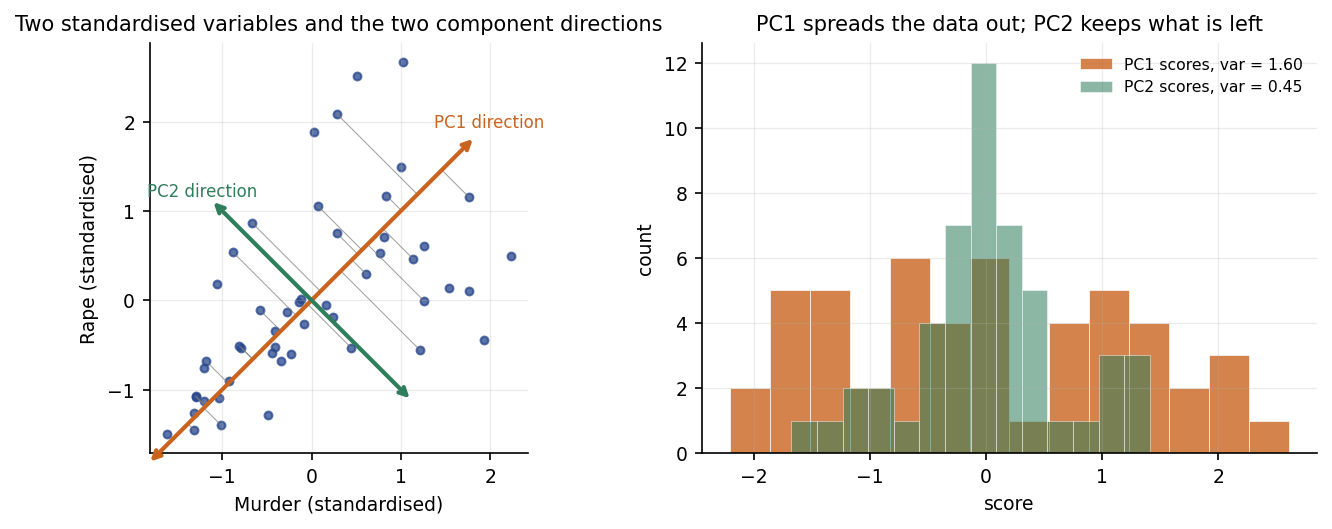
\includegraphics[width=0.92\textwidth,height=0.48\textheight,keepaspectratio]{ch12_pc1_direction.png}
  \end{center}
  \begin{takeaway}
    Murder and Rape (standardised, $r=0.564$) are stretched along the $45^\circ$ line. PC1
    points there and its scores have variance $1.60$; PC2 is forced perpendicular and gets
    only $0.45$. The grey stubs are the projections PC1 keeps --- the shortest possible
    ones, which is the same thing as the widest possible spread.
  \end{takeaway}
\end{frame}

\begin{frame}{Two variables by hand: the whole of PCA in one calculation}
  \footnotesize
  \begin{numexample}[{{Murder and Rape, standardised, $r=0.564$}}]
    The correlation matrix is $\begin{pmatrix}1 & r\\ r & 1\end{pmatrix}$. Its eigenvectors
    are always $\tfrac{1}{\sqrt2}(1,1)^\top$ and $\tfrac{1}{\sqrt2}(1,-1)^\top$, with
    eigenvalues
    \[
      \lambda_1 = 1+r = 1.564, \qquad \lambda_2 = 1-r = 0.436 ,
      \qquad \lambda_1+\lambda_2 = 2 = p .
    \]
    So $\mathrm{PVE}_1=\tfrac{1+r}{2}=78.2\%$ and $\mathrm{PVE}_2=\tfrac{1-r}{2}=21.8\%$.
    (The previous slide's $1.60$ and $0.45$ are the same two eigenvalues computed with the
    $n-1$ divisor: $\tfrac{50}{49}\times1.564=1.60$. The ratio, and so the PVE, is identical.)
  \end{numexample}
  \begin{takeaway}
    Every fact about PCA is visible here: the loadings are a \emph{direction}
    ($0.707,0.707$), the components are orthogonal, the eigenvalues sum to the total
    variance, and the more correlated the features, the more the first component captures.
    Uncorrelated features ($r=0$) give $\lambda_1=\lambda_2=1$ --- PCA has nothing to
    find.
  \end{takeaway}
\end{frame}

\begin{frame}{Later components, and why they are orthogonal}
  \footnotesize
  \begin{block}{Definition}
    $\phi_2$ maximises the variance of $z_{i2}=\sum_j\phi_{j2}x_{ij}$ subject to
    $\|\phi_2\|=1$ \emph{and} $\phi_2^\top\phi_1=0$; and so on for $m=3,\dots,p$.
    Consequently
    \[
      \mathrm{Cov}(z_{\cdot 1}, z_{\cdot 2}) = 0,
      \qquad \sum_{m=1}^{p}\lambda_m = \sum_{j=1}^{p}\mathrm{Var}(X_j) .
    \]
  \end{block}
  \begin{readme}
    \begin{itemize}
      \item Orthogonality is imposed as a \emph{constraint}, not discovered: it is what
            makes each component report \emph{new} variance instead of repeating PC1.
      \item Because the score vectors are uncorrelated, PCA \emph{partitions} the total
            variance --- the $\lambda_m$ add up, with no double counting. There are at most
            $\min(n-1,\,p)$ of them with non-zero variance.
    \end{itemize}
  \end{readme}
  \begin{takeaway}
    PCA is a change of axes, not a model: no assumption, no error term, nothing fitted ---
    which is also why nothing can be tested.
  \end{takeaway}
\end{frame}

\begin{frame}{USArrests: the loadings, read as sentences}
  \footnotesize
  \begin{center}
  \begin{tabular}{@{}lrrrr@{}}
    \toprule
    & \textbf{PC1} & \textbf{PC2} & \textbf{PC3} & \textbf{PC4} \\
    \midrule
    Murder    & $0.536$ & $-0.418$ & $-0.341$ & $-0.649$ \\
    Assault   & $0.583$ & $-0.188$ & $-0.268$ & $\ \ 0.743$ \\
    UrbanPop  & $0.278$ & $\ \ 0.873$ & $-0.378$ & $-0.134$ \\
    Rape      & $0.543$ & $\ \ 0.167$ & $\ \ 0.818$ & $-0.089$ \\
    \midrule
    $\lambda_m$ (variance) & $2.480$ & $0.990$ & $0.357$ & $0.173$ \\
    \bottomrule
  \end{tabular}
  \end{center}
  \begin{readme}[{{Reading the first two columns}}]
    \textbf{PC1} loads on Murder, Assault and Rape at roughly equal weight and on UrbanPop
    only half as much: an overall \emph{serious-crime rate}. \textbf{PC2} is almost entirely
    UrbanPop ($0.873$), the crime variables pulling the other way: \emph{urbanisation at a
    given crime level}.
  \end{readme}
  \begin{industry}[{{Finance: the same table for a yield curve}}]
    PCA on daily changes of a government yield curve gives PC1 $=$ all maturities moving
    together (\emph{level}), PC2 $=$ short up / long down (\emph{slope}), PC3 $=$
    \emph{curvature}. Risk limits are set on those three numbers, not on $30$ tenors.
  \end{industry}
\end{frame}

\begin{frame}{The biplot: scores and loadings in one picture}
  \footnotesize
  \begin{center}
    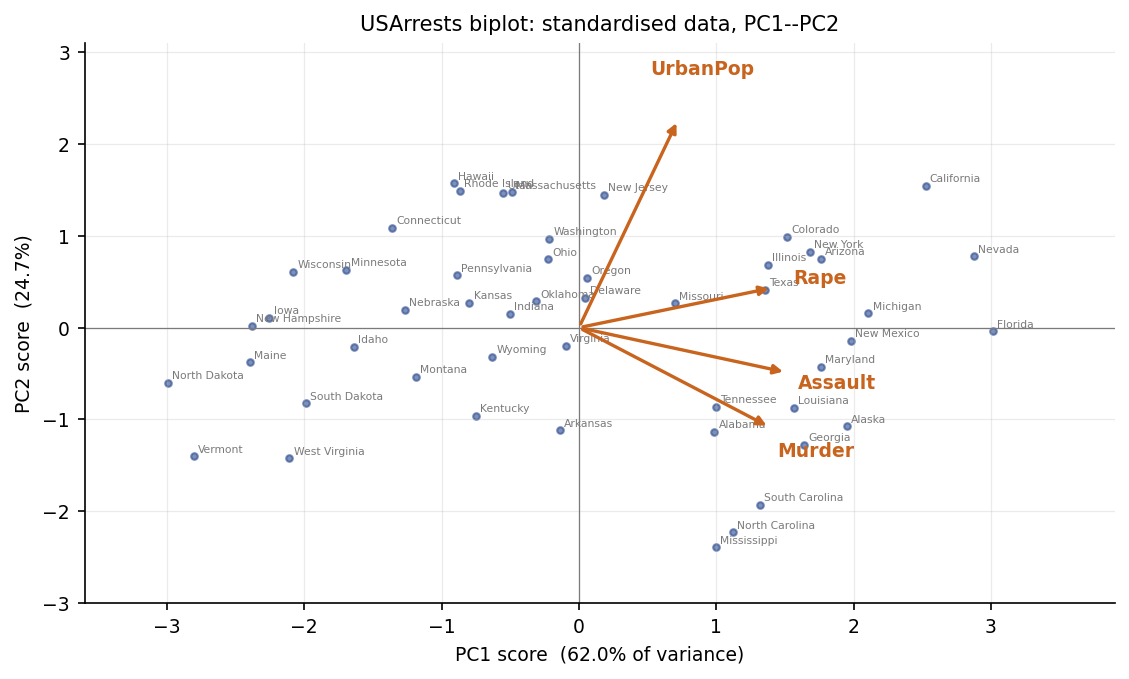
\includegraphics[width=0.90\textwidth,height=0.53\textheight,keepaspectratio]{ch12_biplot.png}
  \end{center}
  \begin{takeaway}
    Florida (PC1 $=3.01$) and Nevada sit at the crime end; North Dakota ($-2.99$) and
    Vermont at the quiet end. Hawaii and California are both high on PC2 (urban); Mississippi
    is lowest ($-2.39$) --- high crime, rural.
  \end{takeaway}
\end{frame}

\begin{frame}{How to read a biplot --- and how not to}
  \footnotesize
  \begin{readme}[{{Four reading rules}}]
    \begin{enumerate}
      \item \textbf{Points} are observations in the plane of the first two scores; nearby
            points have similar profiles \emph{as far as PC1 and PC2 go}.
      \item \textbf{Arrows} are the loadings: an arrow pointing right means high values of
            that feature push a state to the right.
      \item \textbf{Angles between arrows} approximate correlations --- small angle,
            positively correlated; right angle, roughly uncorrelated (UrbanPop vs Murder,
            $r=0.07$).
      \item \textbf{Arrow length} indicates how well the feature is represented by these
            two components, not how important it is.
    \end{enumerate}
  \end{readme}
  \begin{mistake}
    Reading distances between distant points as if the plot were the data. It is a
    \emph{projection}: here it keeps $86.8\%$ of the variance, so $13.2\%$ of the variation
    is not in the picture at all, and two points that look adjacent may differ sharply on
    PC3.
  \end{mistake}
\end{frame}

\begin{frame}{Signs are arbitrary --- your plot may be a mirror image}
  \footnotesize
  \begin{block}{The indeterminacy}
    If $\phi_m$ maximises the variance, so does $-\phi_m$: it is the same direction, and
    $\|-\phi_m\|=1$ too. Flipping it flips every score on that component:
    \[
      \phi_m \mapsto -\phi_m \quad\Longrightarrow\quad z_{im}\mapsto -z_{im}
      \quad\text{for all } i, \qquad \lambda_m \text{ unchanged.}
    \]
  \end{block}
  \begin{numexample}[{{The concrete case in this chapter}}]
    \texttt{scikit-learn} returns PC2 loadings $(-0.418,\,-0.188,\,0.873,\,0.167)$ for
    \texttt{USArrests}. ISLP Figure~12.1 prints $(0.418,\,0.188,\,-0.873,\,-0.167)$.
    Both are correct, and the two biplots are vertical mirror images of each other.
  \end{numexample}
  \begin{mistake}
    Concluding you have made an error because your figure is upside down relative to the
    book. Check the \emph{eigenvalues} and the \emph{absolute} loadings --- those are
    unique. If you must fix a sign for reproducibility, adopt a convention (e.g.\ force the
    largest-magnitude loading of each component to be positive) and state it.
  \end{mistake}
\end{frame}

\begin{frame}{Proportion of variance explained}
  \footnotesize
  \begin{block}{Definition}
    \[
      \boxed{\;\mathrm{PVE}_m=\frac{\lambda_m}{\sum_{m'=1}^{p}\lambda_{m'}}
      =\frac{\sum_{i=1}^{n}z_{im}^{2}}{\sum_{j=1}^{p}\sum_{i=1}^{n}x_{ij}^{2}} ,
      \qquad \sum_{m=1}^{p}\mathrm{PVE}_m=1 .\;}
    \]
  \end{block}
  \begin{readme}
    \begin{itemize}
      \item Numerator: variation the $m$-th component accounts for. Denominator: total
            variation in the (centred) data. On \emph{standardised} data the denominator is
            exactly $np$ and $\sum_m\lambda_m=p$ --- for \texttt{USArrests}, $\lambda$ sums
            to $4$ and the total sum of squares is $50\times4=200$.
      \item Cumulative PVE $=\sum_{m\le M}\mathrm{PVE}_m$ is what you report when you keep
            $M$ components. Its complement $1-\sum_{m\le M}\mathrm{PVE}_m$ is exactly the
            fraction of squared error left when the data is rebuilt from those components,
            because PCA \emph{is} the best rank-$M$ approximation (\emph{appendix}).
    \end{itemize}
  \end{readme}
  \begin{takeaway}
    PVE is a descriptive statistic of \emph{this} data set: not an out-of-sample quantity,
    and never a statement that the components are ``right''.
  \end{takeaway}
\end{frame}

\begin{frame}{The scree plot --- and why choosing $M$ is a judgement call}
  \footnotesize
  \begin{center}
    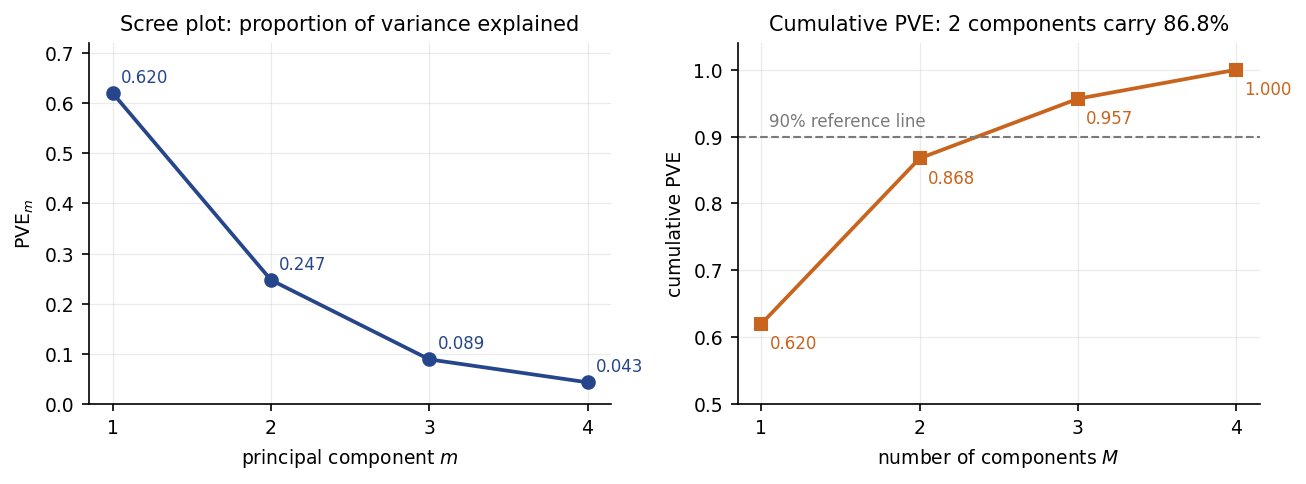
\includegraphics[width=0.94\textwidth,height=0.48\textheight,keepaspectratio]{ch12_scree.png}
  \end{center}
  \begin{takeaway}
    $\mathrm{PVE}=(0.620,\,0.247,\,0.089,\,0.043)$: two components carry $86.8\%$, so a
    two-dimensional picture of the $50$ states is defensible. The ``elbow'' at $m=2$ is a
    kink in a curve, not a test --- there is no held-out quantity that turns $M=2$ into the
    right answer, and $M=3$ ($95.7\%$) is equally defensible.
  \end{takeaway}
\end{frame}

% ------------------------------------------------------------
\begin{frame}{Exercise 12.2 --- PCA from a $2\times2$ correlation matrix [Math]}
\begin{exercise}
  Two standardised features have correlation $r=0.80$ (this is the real
  Murder--Assault correlation in \texttt{USArrests}, to two decimals), so their
  correlation matrix is
  \[
    \mathbf{R}=\begin{pmatrix}1 & 0.8\\ 0.8 & 1\end{pmatrix}.
  \]
  \begin{enumerate}
    \item Find both eigenvalues of $\mathbf{R}$ and the corresponding normalised loading
          vectors.
    \item Compute $\mathrm{PVE}_1$ and $\mathrm{PVE}_2$.
    \item An observation has standardised values $(x_1,x_2)=(1.5,\,1.0)$. Compute its two
          scores.
    \item State what changes if you replace $\phi_1$ by $-\phi_1$.
  \end{enumerate}
\end{exercise}
\end{frame}

\begin{frame}{Solution --- Exercise 12.2}
  \footnotesize
\begin{solutionbox}
  \textbf{Part 1 --- eigen-decomposition.} For $\begin{pmatrix}1&r\\r&1\end{pmatrix}$,
  $\det(\mathbf{R}-\lambda I)=(1-\lambda)^2-r^2=0$, so $1-\lambda=\pm r$ and
  \[
    \lambda_1=1+r=1.8,\qquad \lambda_2=1-r=0.2 .
  \]
  Substituting $\lambda_1$ gives $-0.8\phi_1+0.8\phi_2=0$, i.e.\ $\phi_1=\phi_2$; normalising,
  \[
    \phi_1=\tfrac{1}{\sqrt2}(1,1)^\top=(0.707,\,0.707)^\top,\qquad
    \phi_2=\tfrac{1}{\sqrt2}(1,-1)^\top=(0.707,\,-0.707)^\top .
  \]
  \textbf{Part 2 --- PVE.} Total variance $=\lambda_1+\lambda_2=2=p$, so
  $\mathrm{PVE}_1=1.8/2=90\%$ and $\mathrm{PVE}_2=0.2/2=10\%$.

  \medskip
  \textbf{Part 3 --- scores.}
  $z_1=0.707(1.5)+0.707(1.0)=0.707(2.5)=1.768$ and
  $z_2=0.707(1.5)-0.707(1.0)=0.707(0.5)=0.354$.
  This state is well above average on both features, so it is far out on the ``overall
  level'' component and only slightly off the ``difference'' component.

  \medskip
  \textbf{Part 4 --- sign flip.} $\lambda_1$, $\mathrm{PVE}_1$ and all distances are
  unchanged; every score on PC1 changes sign, so $z_1=-1.768$. The picture is mirrored,
  the analysis is identical.
\end{solutionbox}
\end{frame}

\begin{frame}{Scaling is not optional --- look at the raw variances}
  \footnotesize
  \begin{center}
    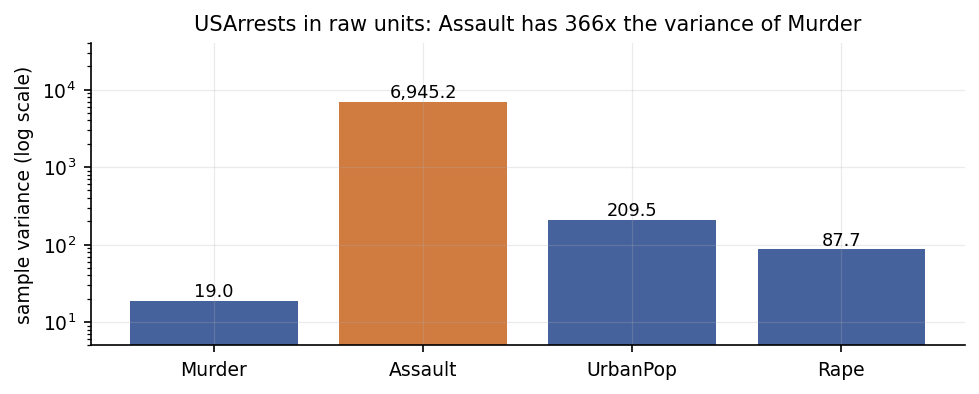
\includegraphics[width=0.80\textwidth,height=0.34\textheight,keepaspectratio]{ch12_variances.png}
  \end{center}
  \begin{numexample}[{{Why PCA cannot ignore this}}]
    \texttt{Assault} is counted per $100\,000$ and \texttt{Murder} is too, but murders are
    rarer: variances are $6945.2$ and $19.0$, a factor of $366$. PCA maximises variance,
    so on raw data the first component has almost no choice but to be Assault.
  \end{numexample}
  \begin{takeaway}
    Recording \texttt{Assault} per million instead of per $100\,000$ would multiply its
    variance by $100$ and change the answer again. PCA on unstandardised data is a
    statement about \emph{units}, not about the world.
  \end{takeaway}
\end{frame}

\begin{frame}{The same data, standardised and not}
  \footnotesize
  \begin{center}
    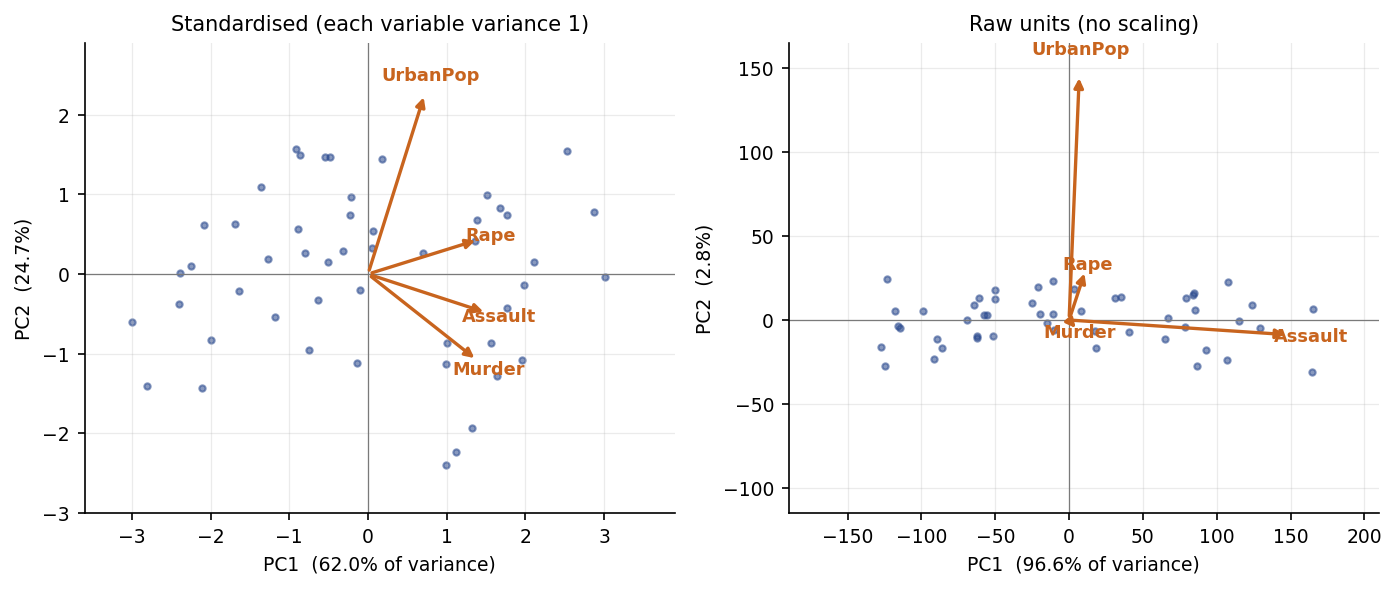
\includegraphics[width=0.94\textwidth,height=0.49\textheight,keepaspectratio]{ch12_scaling.png}
  \end{center}
  \begin{takeaway}
    Left: PC1 takes $62.0\%$ and loads on all four variables ($0.54,0.58,0.28,0.54$).
    Right: PC1 takes $96.6\%$ and is Assault alone (loading $0.995$; Murder gets $0.042$),
    PC2 is UrbanPop, and $99.3\%$ of ``the structure'' is two variables' measurement
    scales. The right-hand panel is not wrong arithmetic --- it is the answer to a
    different, worse question.
  \end{takeaway}
\end{frame}

\begin{frame}{When to standardise, and when not to}
  \footnotesize
  \begin{readme}[{{The rule}}]
    \begin{itemize}
      \item Features in \textbf{different units} (euros, years, counts, percentages)
            $\Rightarrow$ standardise. This is the default, and it means PCA on the
            \emph{correlation} matrix.
      \item Features in the \textbf{same unit and genuinely comparable} --- gene
            expression on one platform, the same price in $30$ maturities, pixels
            $\Rightarrow$ centring alone may be right, because a channel that varies more
            really is more informative.
      \item Never scale a variable up because it ``matters more''. That is a modelling
            choice being smuggled in as a preprocessing step.
    \end{itemize}
  \end{readme}
  \begin{mistake}
    Standardising \emph{after} splitting, or with statistics computed on the full data
    before a split. Fit the scaler where you fit the model --- the Chapter~5 leakage rule
    applies unchanged.
  \end{mistake}
  \begin{labnote}
    \S1 of \texttt{chapter\_12\_lab.ipynb} runs both versions side by side and prints the two
    loading tables.
  \end{labnote}
\end{frame}

% ------------------------------------------------------------
\begin{frame}{Exercise 12.3 --- Scaled vs unscaled PCA on USArrests [Python]}
\begin{exercise}
  Using \texttt{USArrests} ($n=50$, $p=4$):
  \begin{enumerate}
    \item Run PCA on the \textbf{standardised} data. Report the four PVEs and the PC1
          loadings.
    \item Run PCA on the \textbf{centred but unscaled} data. Report the same two things.
    \item Explain the difference by reference to the raw variances, and state which
          analysis you would put in a report.
  \end{enumerate}
\end{exercise}
\begin{labnote}[{{Run this live}}]
  The worked solution sits in \texttt{chapter\_12\_lab.ipynb} under
  \emph{Lecture exercises --- worked Python solutions}: the cell headed
  \emph{Exercise 12.3 --- Scaled vs unscaled PCA on USArrests [Python]}.
\end{labnote}
\end{frame}

\begin{frame}[fragile]{Solution --- Exercise 12.3 (1/2)}
\begin{solutionbox}[{{Solution --- code}}]
\begin{lstlisting}[basicstyle=\ttfamily\scriptsize]
import numpy as np, pandas as pd                       # arrays and frames
from sklearn.decomposition import PCA                  # PCA
from sklearn.preprocessing import StandardScaler       # z-scoring

USA = load('USArrests', index_col=0)                   # 50 states x 4 features
print(USA.var().round(1).to_dict())                    # raw variances: Assault huge

for tag, X in [('scaled',   StandardScaler().fit_transform(USA)),
               ('unscaled', (USA - USA.mean()).values)]:  # centred only
    p = PCA().fit(X)                                   # all 4 components
    print(tag, 'PVE', np.round(p.explained_variance_ratio_, 4))
    print(tag, 'PC1', dict(zip(USA.columns, p.components_[0].round(3))))
\end{lstlisting}
\end{solutionbox}
\end{frame}

\begin{frame}{Solution --- Exercise 12.3 (2/2)}
  \footnotesize
\begin{solutionbox}[{{Solution --- output and interpretation}}]
  \textbf{Raw variances.} Murder $19.0$, Assault $6945.2$, UrbanPop $209.5$, Rape $87.7$.
  \[
    \begin{array}{l|cccc|l}
      & \mathrm{PVE}_1 & \mathrm{PVE}_2 & \mathrm{PVE}_3 & \mathrm{PVE}_4 & \text{PC1 loadings (Mur, Ass, Urb, Rape)}\\ \hline
      \text{scaled}   & 0.6201 & 0.2474 & 0.0891 & 0.0434 & (0.536,\ 0.583,\ 0.278,\ 0.543)\\
      \text{unscaled} & 0.9655 & 0.0278 & 0.0058 & 0.0009 & (0.042,\ 0.995,\ 0.046,\ 0.075)
    \end{array}
  \]
  \textbf{Part 3 --- why.} PCA maximises variance, and \texttt{Assault} carries $366$ times
  the variance of \texttt{Murder} purely because assaults are $22$ times more common. The
  unscaled PC1 is therefore \texttt{Assault} with a rounding error attached, and its
  $96.6\%$ measures the dominance of one column's units, not structure.

  \medskip
  \textbf{What goes in the report.} The \textbf{standardised} analysis --- the four
  variables are on different scales and no one of them deserves $366$ times the weight.
  Say so explicitly in the methods section.
\end{solutionbox}
\begin{mistake}
  Reporting a triumphant ``PC1 explains $96.6\%$ of the variance''. That is the largest
  number available and the least informative one.
\end{mistake}
\end{frame}

\begin{frame}{PCA when $p \gg n$: 1000 genes, 40 samples}
  \footnotesize
  \begin{center}
    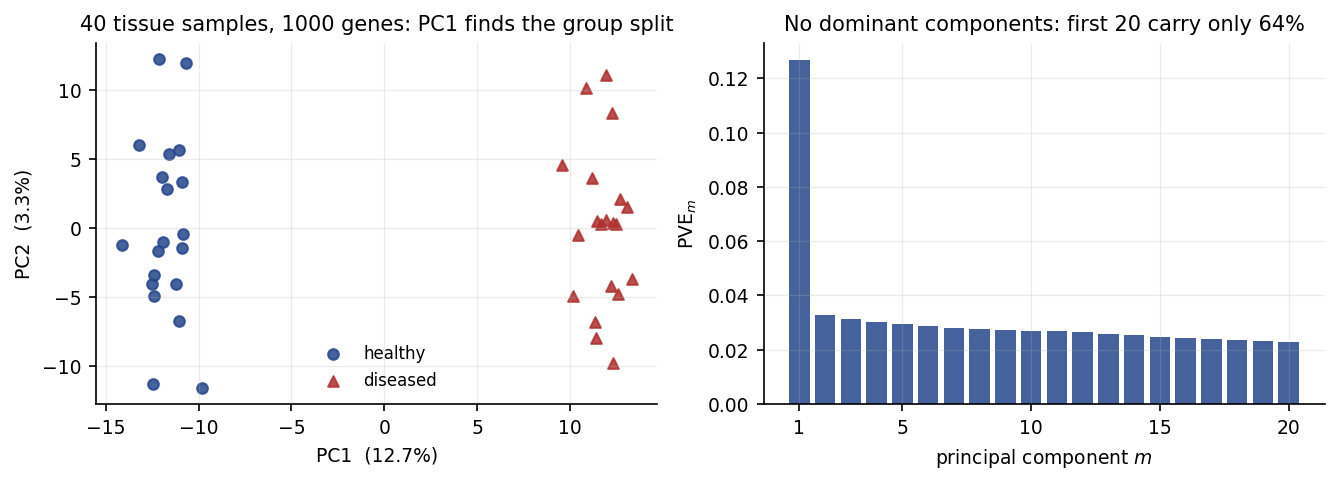
\includegraphics[width=0.94\textwidth,height=0.48\textheight,keepaspectratio]{ch12_gene_pca.png}
  \end{center}
  \begin{takeaway}
    Here PC1 explains only $12.7\%$ --- and separates the $20$ healthy from the $20$
    diseased samples completely (group means $-11.8$ and $+11.8$). A small PVE is not a
    failure: with $p\gg n$ the variance is spread over $39$ components (the first $20$ hold
    $64\%$), and the interesting direction need not be the biggest one.
  \end{takeaway}
\end{frame}

% ============================================================
\section{K-means}
% ============================================================

\begin{frame}{Clustering: what we are asking for}
  \footnotesize
  \begin{readme}[{{The requirement}}]
    A partition $C_1,\dots,C_K$ of the $n$ observations with
    \[
      C_1\cup\cdots\cup C_K=\{1,\dots,n\}, \qquad C_k\cap C_{k'}=\varnothing
      \ \ (k\ne k') ,
    \]
    such that observations inside a cluster are similar and observations in different
    clusters are not.
  \end{readme}
  \begin{takeaway}[{{Two designs, two commitments}}]
    \begin{itemize}
      \item \textbf{$K$-means} --- you must fix $K$ first; you get one flat partition.
      \item \textbf{Hierarchical} --- you fix nothing first; you get a tree and choose $K$
            afterwards by cutting it.
    \end{itemize}
    Neither is a model of how the data arose, so neither can be checked against the data.
  \end{takeaway}
  \begin{industry}[{{Insurance: what ``similar'' has to mean before you start}}]
    Grouping claims by cost alone puts a cheap fraud next to a cheap accident. Choosing the
    features and the distance \emph{is} the analysis; the algorithm is the easy part.
  \end{industry}
\end{frame}

\begin{frame}{The $K$-means objective}
  \scriptsize
  \begin{block}{Rule --- minimise total within-cluster variation}
    \[
      \boxed{\;\min_{C_1,\dots,C_K}\ \sum_{k=1}^{K} W(C_k),
      \quad W(C_k)=\frac{1}{|C_k|}\sum_{i,i'\in C_k}\sum_{j=1}^{p}(x_{ij}-x_{i'j})^{2}
      = 2\sum_{i\in C_k}\sum_{j=1}^{p}(x_{ij}-\bar x_{kj})^{2} \;}
    \]
  \end{block}
  \begin{readme}
    \begin{itemize}
      \item $W(C_k)$ is the average squared Euclidean distance between all pairs inside
            cluster $k$ --- small means tight.
      \item The second equality is an algebraic identity (derived in the appendix): the
            \emph{centroid form}, with $\bar x_{kj}=\frac{1}{|C_k|}\sum_{i\in C_k}x_{ij}$.
            Software reports it without the factor $2$ --- \texttt{sklearn}'s
            \texttt{inertia\_}.
      \item Only the \emph{partition} is optimised; the centroids are a consequence.
    \end{itemize}
  \end{readme}
  \begin{takeaway}
    Because the criterion is squared Euclidean distance, $K$-means implicitly wants
    \textbf{round, equally sized, equally spread} clusters --- and will impose them
    whether or not the data has them.
  \end{takeaway}
\end{frame}

\begin{frame}{The algorithm, step by step}
  \footnotesize
  \begin{block}{Lloyd's algorithm}
    \begin{enumerate}
      \item Assign each observation at random to one of $K$ clusters (or place $K$ initial
            centroids).
      \item Compute the $K$ centroids $\bar x_k$ of the current clusters.
      \item Re-assign every observation to the cluster with the nearest centroid, in
            squared Euclidean distance.
      \item Repeat 2--3 until no assignment changes.
    \end{enumerate}
  \end{block}
  \begin{readme}[{{Why it stops, and what it stops at}}]
    Step~2 cannot increase $\sum_k W(C_k)$ (the mean minimises squared distance) and
    neither can step~3 (each point moves only to a closer centroid). The objective
    therefore decreases monotonically, there are finitely many partitions, so the algorithm
    \textbf{must terminate} --- at a partition no single move can improve. That is a
    \emph{local} optimum.
  \end{readme}
  \begin{takeaway}
    Guaranteed to converge, not guaranteed to be right. There are
    $\sim K^n/K!$ partitions; the algorithm visits a handful.
  \end{takeaway}
\end{frame}

\begin{frame}{USArrests at $K=2$, $3$ and $4$}
  \footnotesize
  \begin{center}
    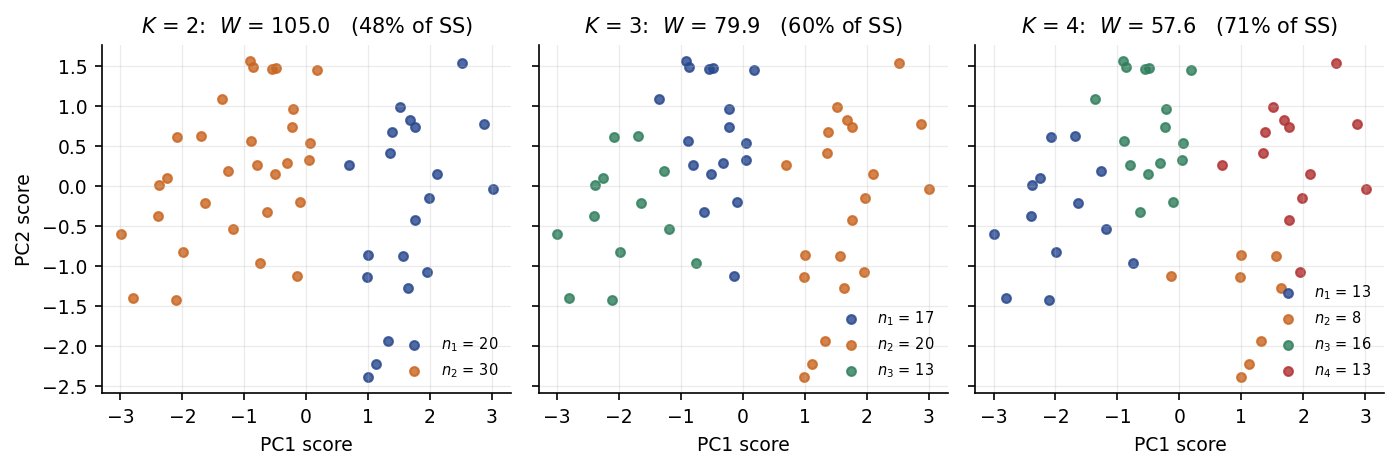
\includegraphics[width=0.98\textwidth,height=0.46\textheight,keepaspectratio]{ch12_kmeans_K.png}
  \end{center}
  \begin{takeaway}
    Total sum of squares is $200$ (standardised, $50\times4$). $W$ falls $200 \to 105.0
    \to 79.9 \to 57.6$, i.e.\ $47\%$, $60\%$, $71\%$ ``explained''. It will keep falling to
    $0$ at $K=50$, so this sequence contains no evidence about which $K$ is right ---
    plotted on PC1--PC2, the clusters are mostly slices of PC1.
  \end{takeaway}
\end{frame}

\begin{frame}{Are the clusters interpretable? The $K=3$ profiles}
  \footnotesize
  \begin{center}
  \begin{tabular}{@{}lrrrrl@{}}
    \toprule
    & \textbf{Murder} & \textbf{Assault} & \textbf{UrbanPop} & \textbf{Rape} & \\
    \midrule
    Cluster 1 ($n=20$) & $12.2$ & $255.2$ & $68.4$ & $29.2$ & high crime, urban \\
    Cluster 2 ($n=17$) & $\ \ 5.8$ & $141.9$ & $72.5$ & $18.8$ & moderate crime, most urban \\
    Cluster 3 ($n=13$) & $\ \ 3.6$ & $\ \ 78.5$ & $52.1$ & $12.2$ & low crime, rural \\
    \midrule
    Overall            & $\ \ 7.8$ & $170.8$ & $65.5$ & $21.2$ & \\
    \bottomrule
  \end{tabular}
  \end{center}
  \begin{readme}[{{The only honest check available on this slide}}]
    Cluster means in the \emph{original units} are how a clustering earns its keep: if the
    three rows read as three recognisable kinds of state, the partition is useful. That is
    interpretability, not validation --- three groups ordered along one crime axis is
    exactly what $K$-means would produce from a single unimodal cloud too.
  \end{readme}
  \begin{industry}[{{Retail: profiling is the deliverable}}]
    Nobody buys a table of cluster labels. The deliverable is this table --- average basket,
    frequency, tenure, margin per segment --- because a campaign is written against it.
  \end{industry}
\end{frame}

\begin{frame}{$K$-means finds a local optimum --- with real numbers}
  \footnotesize
  \begin{center}
    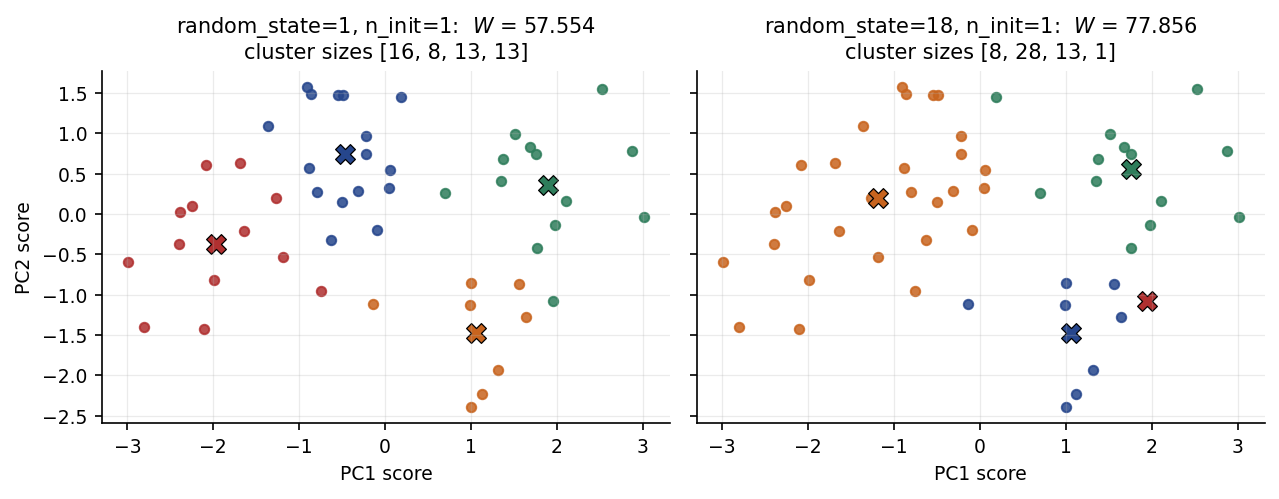
\includegraphics[width=0.92\textwidth,height=0.46\textheight,keepaspectratio]{ch12_local_optima.png}
  \end{center}
  \begin{takeaway}
    Same data, same $K=4$, same code --- only the random start differs
    (\texttt{n\_init=1}). Seed $1$ reaches $W=57.554$ with sizes $(16,8,13,13)$; seed $18$
    stops at $W=77.856$ with sizes $(8,28,13,1)$, having merged two groups and left one
    state alone. Fifteen of the fifty states change cluster (ARI $0.573$), and neither run
    knows the other exists.
  \end{takeaway}
\end{frame}

\begin{frame}{The practical defence: many starts, and say how many}
  \scriptsize
  \begin{numexample}[{{Twenty single-start runs, $K=4$, \texttt{USArrests} standardised}}]
    Seeds $0$--$19$ give, sorted:
    $57.554\,(\times7)$, $57.668\,(\times2)$, $57.673$, $58.207\,(\times3)$,
    $58.242\,(\times3)$, $58.782$, $58.962$, $71.875$, $77.856$ --- \textbf{nine} distinct
    local optima. Thirteen of the twenty runs miss the best value and the worst is $35\%$
    above it; with \texttt{n\_init=50}, $W=57.554$ every time.
  \end{numexample}
  \begin{readme}[{{What to do}}]
    \begin{itemize}
      \item \textbf{Always set \texttt{n\_init} explicitly}, to $20$--$50$. Since
            \texttt{scikit-learn} 1.4 the default is \texttt{n\_init='auto'}, which with the
            default \texttt{k-means++} initialisation means \textbf{one start}:
            \texttt{KMeans(n\_clusters=4, random\_state=0)} on this data returns $W=58.242$,
            not the optimum $57.554$.
      \item Report the objective, \texttt{n\_init} and the seed --- a clustering without them
            is not reproducible. If several starts give \emph{equally good} objectives but
            different partitions, the structure is weak, and that is information too.
      \end{itemize}
  \end{readme}
  \begin{mistake}
    Treating $K$-means as deterministic and comparing two teams' cluster~$3$: even at the
    same optimum the \emph{labels} are arbitrary.
  \end{mistake}
\end{frame}

% ------------------------------------------------------------
\begin{frame}{Exercise 12.4 --- Two local optima on four points [Math]}
\begin{exercise}
  Four observations sit at the corners of a rectangle:
  \[
    x_1=(0,0),\quad x_2=(0,1),\quad x_3=(4,0),\quad x_4=(4,1),
  \]
  and we run $K$-means with $K=2$. Use $W=\sum_k\sum_{i\in C_k}\|x_i-\bar x_k\|^2$
  (\texttt{sklearn}'s \texttt{inertia\_}).
  \begin{enumerate}
    \item Compute $W$ for the \emph{vertical} split $\{x_1,x_2\},\{x_3,x_4\}$.
    \item Compute $W$ for the \emph{horizontal} split $\{x_1,x_3\},\{x_2,x_4\}$.
    \item Show that the horizontal split is a fixed point of the algorithm --- no single
          observation wants to move.
    \item What does this imply about running $K$-means once?
  \end{enumerate}
\end{exercise}
\end{frame}

\begin{frame}{Solution --- Exercise 12.4 (1/2)}
\begin{solutionbox}
  \textbf{Part 1 --- vertical split.} Centroids $(0,0.5)$ and $(4,0.5)$. Each point is
  $0.5$ from its centroid, so
  \[
    W=4\times(0.5)^2=1.0 .
  \]
  \textbf{Part 2 --- horizontal split.} Centroids $(2,0)$ and $(2,1)$. Each point is
  $2$ away in $x_1$ and $0$ in $x_2$:
  \[
    W=4\times 2^2=16.0 .
  \]
  \textbf{Part 3 --- it is stable.} Take $x_1=(0,0)$ under the horizontal split. Squared
  distances to the two centroids are
  \[
    \|x_1-(2,0)\|^2=4 \qquad\text{and}\qquad \|x_1-(2,1)\|^2=4+1=5 .
  \]
  It is already in the nearer cluster, so it stays; by symmetry so does every other point.
  The centroids do not move either, so step~3 changes nothing and the algorithm
  \textbf{terminates here}, reporting $W=16$ --- sixteen times the optimum.
\end{solutionbox}
\end{frame}

\begin{frame}{Solution --- Exercise 12.4 (2/2)}
  \footnotesize
\begin{solutionbox}
  \textbf{Part 4 --- consequence.} A single run of $K$-means can return an arbitrarily bad
  partition and give no sign of it: the algorithm's stopping rule (``no point wants to
  move'') is satisfied at both $W=1$ and $W=16$. Only comparing \emph{several} random
  starts and keeping the lowest $W$ protects you, which is what \texttt{n\_init} does.

  \medskip
  \textbf{Verification in code.} Initialising at $(0,0.5),(4,0.5)$ gives $W=1.0$; at
  $(2,0),(2,1)$ it gives $W=16.0$; \texttt{n\_init=20} returns $1.0$.

  \smallskip
  \textit{Common mistake:} concluding that a \emph{converged} run is a \emph{good} run.
  Convergence is a fact about the algorithm; quality is about $W$, and $W$ is only
  interpretable relative to other starts at the \emph{same} $K$.
\end{solutionbox}
\begin{center}
  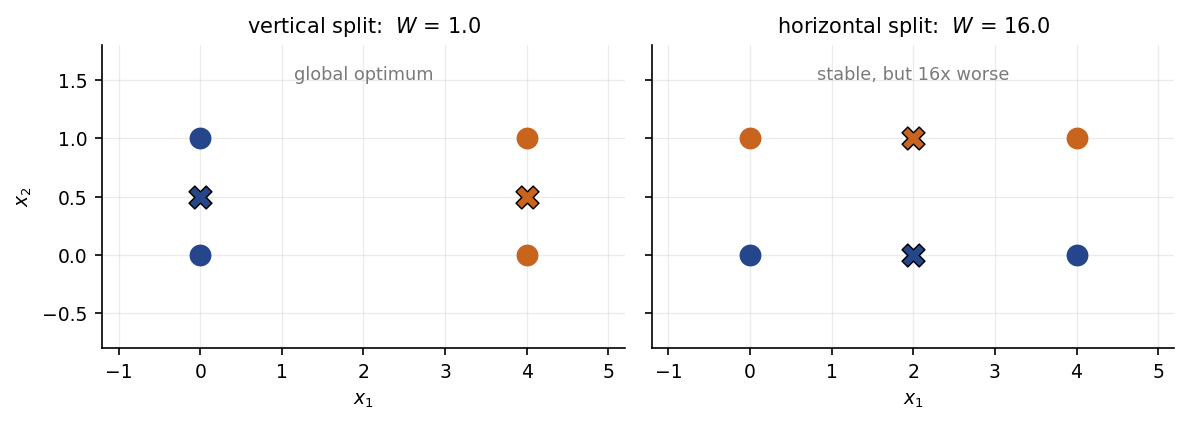
\includegraphics[width=0.70\textwidth,height=0.30\textheight,keepaspectratio]{ch12_x_rectangle.png}
\end{center}
\end{frame}

\begin{frame}{Choosing $K$: what the standard diagnostics can and cannot do}
  \footnotesize
  \begin{center}
    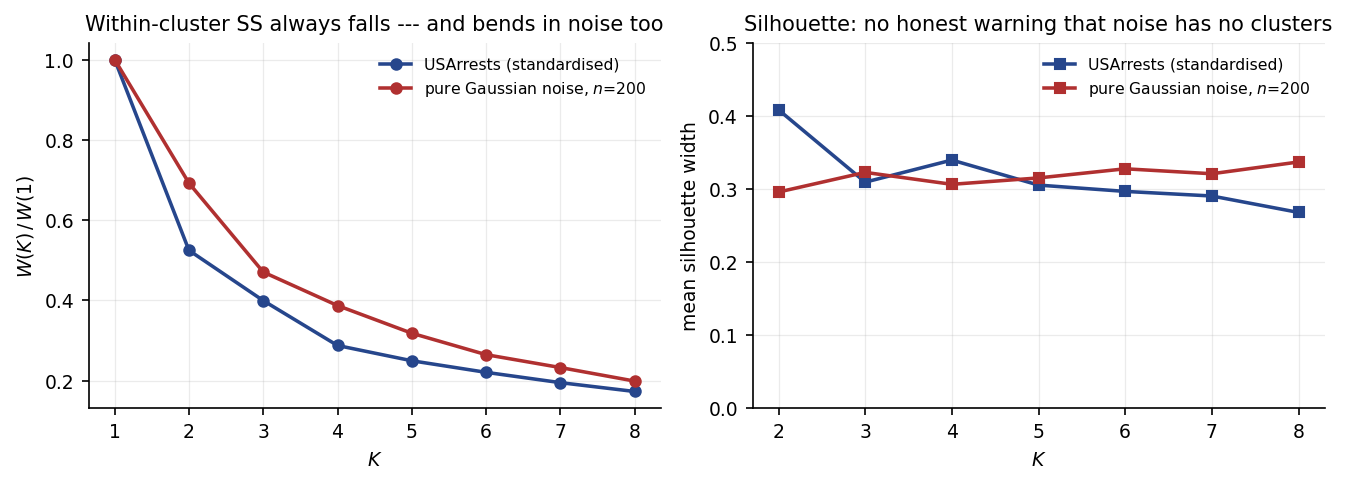
\includegraphics[width=0.94\textwidth,height=0.44\textheight,keepaspectratio]{ch12_choose_K.png}
  \end{center}
  \begin{takeaway}
    Left: $W(K)/W(1)$ falls smoothly for \texttt{USArrests} \emph{and} for $200$ points of
    pure Gaussian noise --- the noise curve bends just as convincingly ($0.69$, $0.47$,
    $0.39$ at $K=2,3,4$). Right: the mean silhouette on noise sits at $0.30$--$0.34$ for
    every $K$ and is \emph{highest at $K=8$}. These diagnostics rank candidate $K$; they
    never say ``there are no clusters''.
  \end{takeaway}
\end{frame}

% ------------------------------------------------------------
\begin{frame}{Extended Exercise 12.1 --- How bad is the local-optimum problem? [Python]}
\begin{longexercise}
  On standardised \texttt{USArrests}, quantify the local-optimum problem instead of
  asserting it.
  \begin{enumerate}
    \item For $K=4$, run $K$-means with \texttt{n\_init=1} for seeds $0,\dots,19$ and
          collect the objective \texttt{inertia\_} and the sorted cluster sizes.
    \item Report how many \emph{distinct} local optima appear, the best and worst
          objective, and the percentage gap between them.
    \item Compare with a single run at \texttt{n\_init=50}, and repeat the whole exercise
          at $K=8$.
    \item State the reporting rule you would impose on a team from these numbers.
  \end{enumerate}
\end{longexercise}
\begin{labnote}[{{Run this live}}]
  The worked solution sits in \texttt{chapter\_12\_lab.ipynb} under
  \emph{Lecture exercises --- worked Python solutions}: the cell headed
  \emph{Extended Exercise 12.1 --- How bad is the local-optimum problem? [Python]}.
\end{labnote}
\end{frame}

\begin{frame}[fragile]{Solution --- Extended Exercise 12.1 (1/2)}
\begin{solutionbox}[{{Solution --- code}}]
\begin{lstlisting}[basicstyle=\ttfamily\scriptsize]
from sklearn.cluster import KMeans
from sklearn.preprocessing import StandardScaler

Xs = StandardScaler().fit_transform(load('USArrests', index_col=0))

for K in (4, 8):
    runs = [KMeans(n_clusters=K, n_init=1, random_state=s).fit(Xs)
            for s in range(20)]                  # 20 single-start runs
    w = np.array([r.inertia_ for r in runs])     # the objective, once per seed
    best = KMeans(n_clusters=K, n_init=50, random_state=0).fit(Xs).inertia_
    print(f'K={K}: {len(np.unique(w.round(3)))} optima  min={w.min():.3f}  '
          f'max={w.max():.3f}  gap={100*(w.max()/w.min()-1):.1f}%  '
          f'n_init=50 -> {best:.3f}')
    print('  best / worst sizes', sorted(np.bincount(runs[w.argmin()].labels_)),
          sorted(np.bincount(runs[w.argmax()].labels_)))
\end{lstlisting}
\end{solutionbox}
\end{frame}

\begin{frame}{Solution --- Extended Exercise 12.1 (2/2)}
  \footnotesize
\begin{solutionbox}[{{Solution --- output and the reporting rule}}]
  \textbf{Printout.}
  \begin{center}\ttfamily\footnotesize
  K=4: 9 optima\ \ min=57.554\ \ max=77.856\ \ gap=35.3\%\ \ n\_init=50 -> 57.554\\[1pt]
  \ \ best / worst sizes [8, 13, 13, 16] [1, 8, 13, 28]\\[3pt]
  K=8: 20 optima\ \ min=36.551\ \ max=40.965\ \ gap=12.1\%\ \ n\_init=50 -> 34.636
  \end{center}
  \begin{itemize}
    \item \textbf{Parts 1--2.} At $K=4$, twenty starts land on \emph{nine} different local
          optima and the worst is $35.3\%$ above the best. The failure is structural, not a
          rounding issue: the worst run returns sizes $(1,8,13,28)$ --- one state alone in
          its own cluster and more than half in another --- against $(8,13,13,16)$ for the
          best.
    \item \textbf{Part 3.} At $K=8$ all twenty starts give twenty \emph{different} values
          ($36.551$ to $40.965$) and \emph{none} of them reaches the \texttt{n\_init=50}
          value of $34.636$. More clusters means a rougher objective surface and more
          places to get stuck --- exactly where a single run is least trustworthy.
    \item \textbf{Part 4 --- the rule.} Every reported clustering states $K$, the
          dissimilarity, the scaling, \texttt{n\_init} ($\ge 20$), the seed and the
          achieved objective. Two runs whose $W$ differs are not two opinions; one of them
          is simply worse.
  \end{itemize}
\end{solutionbox}
\end{frame}

% ============================================================
\section{Hierarchical}
% ============================================================

\begin{frame}{Hierarchical clustering: commit to nothing in advance}
  \footnotesize
  \begin{readme}[{{What it gives you that $K$-means does not}}]
    \begin{itemize}
      \item No $K$ is chosen before fitting. One tree contains the partition for
            \emph{every} $K$ from $1$ to $n$.
      \item The partitions are \textbf{nested}: the $3$-cluster solution always refines the
            $2$-cluster one.
      \item It needs only a table of pairwise dissimilarities, so it works where no
            ``mean'' exists (text, categorical profiles, correlations).
      \item But nesting is a real \emph{restriction}: if the best two-group split of your
            customers is by country and the best three-group split is by product, no
            dendrogram shows both.
    \end{itemize}
  \end{readme}
  \begin{block}{Bottom-up (agglomerative) algorithm}
    \begin{enumerate}
      \item Start with $n$ clusters of one observation each and all $\binom{n}{2}$
            pairwise dissimilarities.
      \item Fuse the two \emph{least dissimilar} clusters; record the dissimilarity as the
            \textbf{height} of that fusion.
      \item Recompute dissimilarities between the new cluster and the rest using the chosen
            \textbf{linkage}; repeat until one cluster remains.
    \end{enumerate}
  \end{block}
\end{frame}

\begin{frame}{Reading a dendrogram}
  \footnotesize
  \begin{readme}[{{Three rules, in order of importance}}]
    \begin{enumerate}
      \item \textbf{Height is everything.} Two observations are similar if the height at
            which their branches \emph{first join} is low. Read the vertical axis.
      \item \textbf{Horizontal position means nothing.} A dendrogram has $2^{n-1}$ equally
            valid drawings; the ordering of leaves is a plotting choice.
      \item \textbf{Cutting} at a height gives a partition; the number of vertical lines the
            cut crosses is $K$.
    \end{enumerate}
  \end{readme}
  \begin{takeaway}
    In the complete-linkage tree overleaf Alaska is drawn immediately next to Alabama, yet
    the two only join at height $3.29$; Alabama and \emph{Louisiana} join at $0.78$, and
    Alabama and Iowa not until $6.14$. Adjacency lied; the heights did not.
  \end{takeaway}
  \begin{industry}[{{Pharma: reading a heatmap dendrogram in a paper}}]
    Expression heatmaps put a dendrogram on each margin. Reviewers check the \emph{merge
    heights} and whether the reported subtypes survive a change of linkage --- adjacent
    columns prove nothing.
  \end{industry}
\end{frame}

\begin{frame}{Cutting the tree chooses $K$ --- after you have seen it}
  \footnotesize
  \begin{center}
    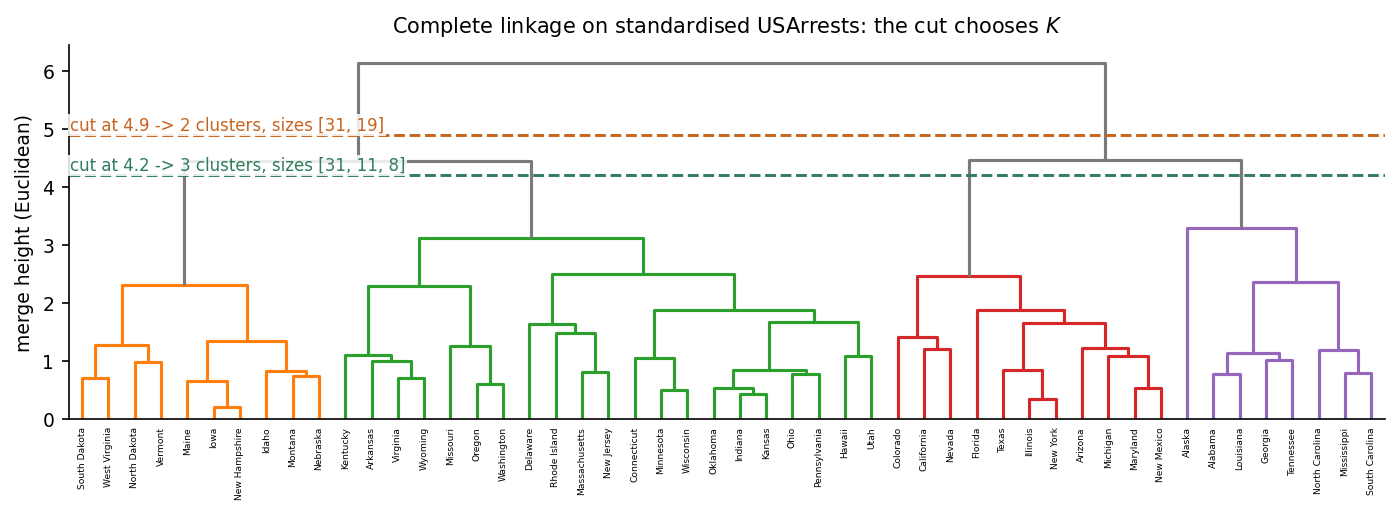
\includegraphics[width=0.98\textwidth,height=0.48\textheight,keepaspectratio]{ch12_dendro_cut.png}
  \end{center}
  \begin{takeaway}
    Complete linkage on standardised \texttt{USArrests}: cutting at $4.9$ gives $2$
    clusters of sizes $(31,19)$; cutting at $4.2$ gives $3$ of sizes $(31,11,8)$. Both cuts
    are legitimate. Choosing the height \emph{after} looking at the tree is exactly the
    selection problem Chapter~13 formalises --- and here there is no $p$-value to correct.
  \end{takeaway}
\end{frame}

\begin{frame}{The same tree, drawn two ways}
  \begin{center}
    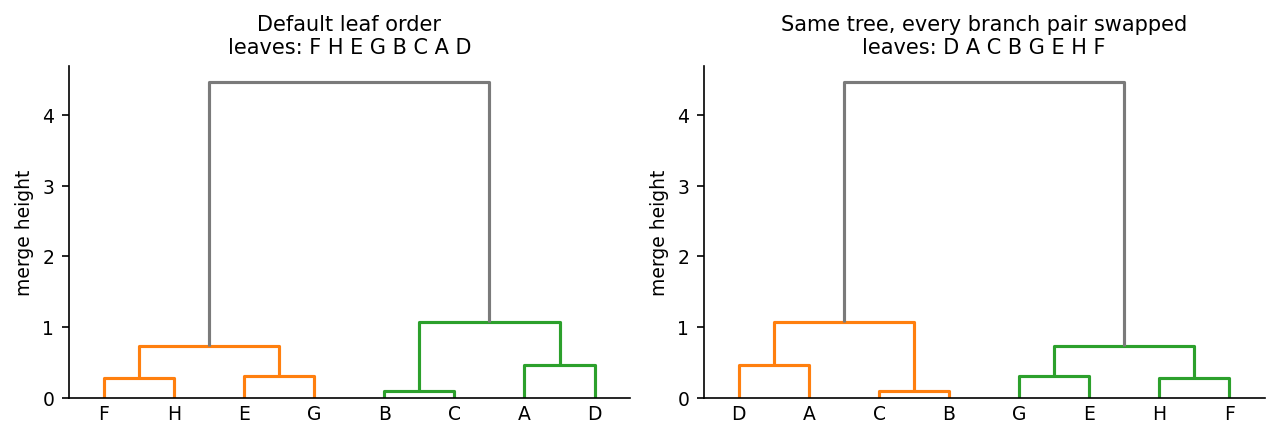
\includegraphics[width=0.94\textwidth,height=0.46\textheight,keepaspectratio]{ch12_dendro_swap.png}
  \end{center}
  \begin{mistake}[{{The commonest dendrogram error}}]
    Both panels are the \emph{identical} clustering: every merge height is the same, only
    the left/right order of each branch pair was swapped. Leaf order changes from
    \texttt{F H E G B C A D} to \texttt{D A C B G E H F}. In the left panel $G$ looks
    ``next to'' $B$; in the right it does not. If your conclusion changes between these two
    pictures, your conclusion was about the drawing.
  \end{mistake}
\end{frame}

% ------------------------------------------------------------
\begin{frame}{Exercise 12.5 --- Reading a dendrogram [Concept]}
\begin{exercise}
  A dendrogram over five observations has fusion heights: $\{A,B\}$ at $0.4$;
  $\{C,D\}$ at $0.6$; $\{A,B\}$ with $E$ at $1.5$; $\{A,B,E\}$ with $\{C,D\}$ at $2.8$.
  \begin{enumerate}
    \item Which pair of observations is the most similar, and which observation is the last
          individual leaf to join a cluster?
    \item Give the partitions obtained by cutting at heights $0.5$, $1.0$, $2.0$ and
          $3.0$.
    \item In one drawing $E$ appears immediately to the left of $C$. What, if anything,
          does that tell you about $E$ and $C$?
    \item Why is ``cut wherever the biggest vertical gap is'' not a validation procedure?
  \end{enumerate}
\end{exercise}
\end{frame}

\begin{frame}{Solution --- Exercise 12.5}
\begin{solutionbox}
  \textbf{Part 1.} $A$ and $B$ fuse lowest ($0.4$), so they are the most similar pair. The
  last individual leaf to join anything is $E$, at height $1.5$ --- compared with $0.4$ for
  $A,B$ and $0.6$ for $C,D$, so $E$ is the most isolated single observation. (The fusion at
  $2.8$ joins two \emph{clusters}, not a leaf.)

  \medskip
  \textbf{Part 2 --- cuts.}
  \[
    \begin{array}{c|l|c}
      \text{height} & \text{partition} & K\\ \hline
      0.5 & \{A,B\},\{C\},\{D\},\{E\} & 4\\
      1.0 & \{A,B\},\{C,D\},\{E\} & 3\\
      2.0 & \{A,B,E\},\{C,D\} & 2\\
      3.0 & \{A,B,C,D,E\} & 1
    \end{array}
  \]
  \textbf{Part 3.} Nothing at all. Horizontal adjacency is an artefact of the drawing; $E$
  and $C$ first share a cluster only at height $2.8$, the largest fusion in the tree, so
  they are in fact among the \emph{least} similar pairs.

  \medskip
  \textbf{Part 4.} The gap is computed from the same data that produced the tree, so it
  cannot be contradicted by it: any data set, structured or not, has a largest gap. It is a
  reasonable heuristic for \emph{proposing} $K$ and no evidence that $K$ clusters exist.
\end{solutionbox}
\end{frame}

\begin{frame}{Linkage: how to measure the distance between two \emph{groups}}
  \footnotesize
  \begin{block}{The four classical choices, for groups $A$ and $B$}
    \[
      \begin{array}{ll}
        \textbf{Complete} & d(A,B)=\max_{i\in A,\,i'\in B} d(i,i') \\[2pt]
        \textbf{Single}   & d(A,B)=\min_{i\in A,\,i'\in B} d(i,i') \\[2pt]
        \textbf{Average}  & d(A,B)=\dfrac{1}{|A||B|}\sum_{i\in A}\sum_{i'\in B} d(i,i') \\[4pt]
        \textbf{Centroid} & d(A,B)=\|\bar x_A - \bar x_B\|^2
      \end{array}
    \]
  \end{block}
  \begin{readme}[{{What each one does to the shape of the answer}}]
    \begin{itemize}
      \item \textbf{Complete} --- a cluster is only as good as its worst pair: compact,
            similarly sized, balanced clusters.
      \item \textbf{Single} --- one close pair is enough to fuse: produces long chains and
            strips off singletons (\emph{chaining}).
      \item \textbf{Average} --- the compromise; with complete, the usual default.
      \item \textbf{Centroid} --- used in genomics, but can produce an \textbf{inversion}
            (a fusion \emph{lower} than one of its children), which makes the picture hard
            to read.
    \end{itemize}
  \end{readme}
\end{frame}

\begin{frame}{One data set, two linkages, two different answers}
  \footnotesize
  \begin{center}
    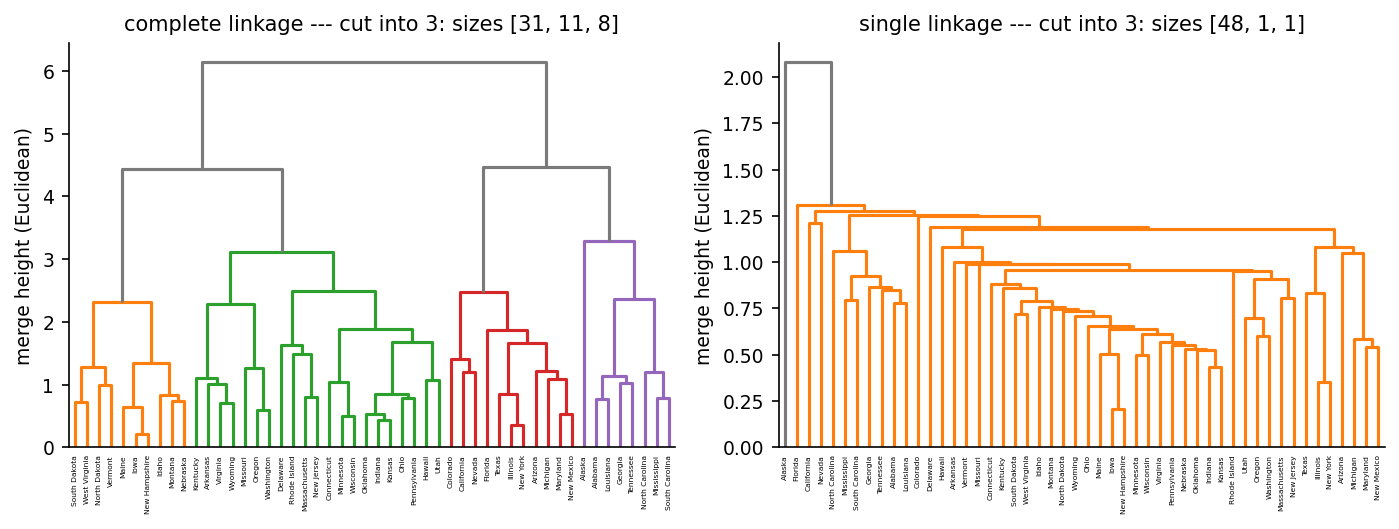
\includegraphics[width=0.98\textwidth,height=0.46\textheight,keepaspectratio]{ch12_dendro_linkage.png}
  \end{center}
  \begin{takeaway}
    Identical data, identical Euclidean distances, identical cut into $3$. Complete linkage
    returns balanced clusters of sizes $(31,11,8)$; single linkage returns
    $(48,1,1)$ --- it peels off Alaska and Florida one at a time and calls the other $48$
    states one cluster. The agreement between the two partitions is an adjusted Rand index
    of $0.079$: essentially none.
  \end{takeaway}
\end{frame}

\begin{frame}{How much does the linkage choice matter? Quantify it}
  \scriptsize
  \begin{numexample}[{{Standardised \texttt{USArrests}, Euclidean, cut into $K=3$}}]
    \[
      \begin{array}{l|c|c|c}
        \text{linkage} & \text{sizes} & \text{tallest fusion} & \text{ARI vs complete}\\ \hline
        \text{complete} & (31,11,8) & 6.14 & 1.000 \\
        \text{average}  & (30,19,1) & 3.36 & 0.784 \\
        \text{single}   & (48,1,1)  & 2.08 & 0.079 \\
        \text{Ward}     & (19,12,19)& 13.65& 0.465
      \end{array}
    \]
    Centroid linkage reproduces average exactly here. $K$-means at $K=3$ agrees with
    complete at ARI $0.394$, average $0.607$, Ward $0.878$ --- and single $-0.013$, worse
    than chance.
  \end{numexample}
  \begin{takeaway}
    Five defensible methods, five different partitions of the same $50$ states, no quantity
    in the data ranking them. The linkage is a \textbf{modelling assumption about cluster
    shape}: choose it before you see the answer, and say which you chose.
  \end{takeaway}
  \begin{industry}[{{Banking: why the choice goes into the model documentation}}]
    A reviewer must reproduce the segments exactly, so the distance, the linkage and the cut
    height are all named --- single linkage would quietly turn $19$ segments into $1$ plus
    $18$ singletons.
  \end{industry}
\end{frame}

% ------------------------------------------------------------
\begin{frame}{Exercise 12.6 --- Complete vs single linkage by hand [Math]}
\begin{exercise}
  Four observations have the dissimilarity matrix
  \[
    D=\begin{pmatrix}
      0 & 0.30 & 0.40 & 0.70\\
      0.30 & 0 & 0.50 & 0.80\\
      0.40 & 0.50 & 0 & 0.45\\
      0.70 & 0.80 & 0.45 & 0
    \end{pmatrix}.
  \]
  \begin{enumerate}
    \item Build the dendrogram under \textbf{complete} linkage, giving every fusion height.
    \item Build it under \textbf{single} linkage.
    \item In each case, which clusters result from cutting the tree so that two clusters
          remain?
    \item Explain the difference in terms of the definitions.
  \end{enumerate}
\end{exercise}
\end{frame}

\begin{frame}{Solution --- Exercise 12.6 (1/2)}
\begin{solutionbox}[{{Solution --- complete linkage}}]
  \textbf{Step 1.} The smallest entry is $d(1,2)=0.30$: fuse $\{1,2\}$ at height
  $\mathbf{0.30}$.

  \medskip
  \textbf{Step 2 --- update with the maximum.}
  \[
    d(\{1,2\},3)=\max(0.40,0.50)=0.50,\qquad
    d(\{1,2\},4)=\max(0.70,0.80)=0.80,\qquad
    d(3,4)=0.45 .
  \]
  The smallest is now $0.45$: fuse $\{3,4\}$ at height $\mathbf{0.45}$.

  \medskip
  \textbf{Step 3.} $d(\{1,2\},\{3,4\})=\max(0.40,0.50,0.70,0.80)=0.80$: the final fusion
  is at height $\mathbf{0.80}$.

  \medskip
  \textbf{Tree.} $\{1,2\}$ at $0.30$, $\{3,4\}$ at $0.45$, root at $0.80$.
  Cutting below $0.80$ leaves \textbf{two clusters: $\{1,2\}$ and $\{3,4\}$.}
\end{solutionbox}
\end{frame}

\begin{frame}{Solution --- Exercise 12.6 (2/2)}
  \footnotesize
\begin{solutionbox}[{{Solution --- single linkage, and the comparison}}]
  \textbf{Step 1.} Same first fusion: $\{1,2\}$ at height $\mathbf{0.30}$.

  \medskip
  \textbf{Step 2 --- update with the minimum.}
  \[
    d(\{1,2\},3)=\min(0.40,0.50)=0.40,\qquad
    d(\{1,2\},4)=\min(0.70,0.80)=0.70,\qquad
    d(3,4)=0.45 .
  \]
  Now the smallest is $0.40$, so observation $3$ joins $\{1,2\}$ at height $\mathbf{0.40}$
  --- \emph{before} $3$ and $4$ ever meet.

  \medskip
  \textbf{Step 3.} $d(\{1,2,3\},4)=\min(0.70,0.80,0.45)=0.45$: final fusion at
  $\mathbf{0.45}$. Cutting below it leaves \textbf{$\{1,2,3\}$ and $\{4\}$.}

  \medskip
  \textbf{Part 4 --- why.} Complete linkage judged $\{1,2\}$ and $3$ by their \emph{worst}
  pair ($0.50$), which let $3$ and $4$ pair up first. Single linkage judged them by their
  \emph{best} pair ($0.40$) and chained $3$ onto $\{1,2\}$, leaving $4$ alone. Same
  distances, incompatible answers --- and single linkage's heights are systematically lower,
  so its tree looks flatter.

  \smallskip
  \textit{Common mistake:} recomputing group distances from the \emph{original} matrix each
  round, or averaging the fused rows when you meant to take a maximum.
\end{solutionbox}
\end{frame}

\begin{frame}{The dissimilarity measure: often the bigger decision}
  \footnotesize
  \begin{block}{Two common choices}
    \[
      \underbrace{d(i,i')=\sum_{j=1}^{p}(x_{ij}-x_{i'j})^{2}}_{\text{squared Euclidean: cares about \emph{level}}}
      \qquad\qquad
      \underbrace{d(i,i')=1-r_{ii'}}_{\text{correlation-based: cares about \emph{shape}}}
    \]
    where $r_{ii'}$ is the correlation across the $p$ features between observation $i$'s
    and $i'$'s profiles.
  \end{block}
  \begin{readme}[{{When they disagree}}]
    Two shoppers who buy the same categories in the same proportions but one spends ten
    times more are \emph{far} in Euclidean distance and \emph{identical} in correlation
    distance. Which is right depends entirely on the question: total spend, or taste?
  \end{readme}
  \begin{takeaway}
    Standardising the features is itself part of this choice, because scaling changes every
    Euclidean distance. Also note $1-r$ needs $p\ge 3$ to mean anything: with $p=2$ every
    correlation between two profiles is $\pm 1$.
  \end{takeaway}
\end{frame}

\begin{frame}{The measure can matter more than the algorithm}
  \footnotesize
  \begin{center}
    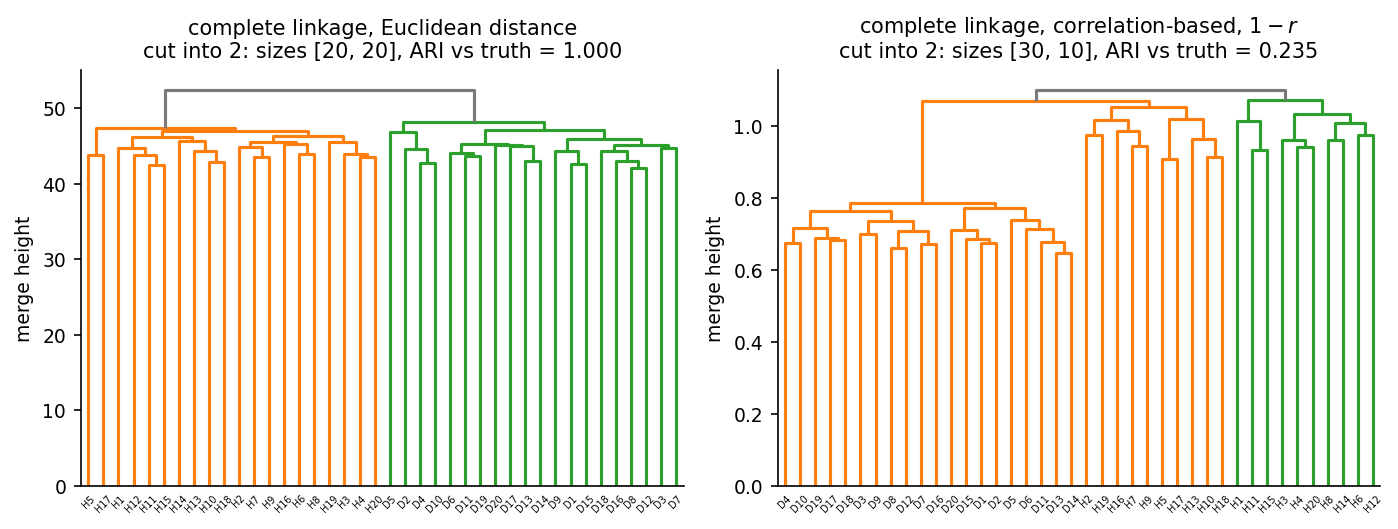
\includegraphics[width=0.98\textwidth,height=0.41\textheight,keepaspectratio]{ch12_corr_vs_eucl.png}
  \end{center}
  \begin{takeaway}
    $40$ tissue samples, $1000$ genes, $20$ healthy and $20$ diseased. With
    \textbf{Euclidean} distance, complete linkage recovers the two groups exactly
    (sizes $20{+}20$, ARI $=1.000$) --- and so do single and average linkage. With
    \textbf{$1-r$} the same linkage returns $(30,10)$, ARI $=0.235$; average gives $0.188$
    and single gives $0.000$. Here the group difference is a shift in $500$ genes' levels,
    which correlation deliberately discards. Swapping the linkage changed little; swapping
    the \emph{distance} destroyed the signal.
  \end{takeaway}
\end{frame}

\begin{frame}{$K$-means or hierarchical? A decision table}
  \begin{center}\footnotesize
  \begin{tabular}{@{}p{3.5cm}p{4.6cm}p{4.6cm}@{}}
    \toprule
     & \textbf{$K$-means} & \textbf{Hierarchical} \\
    \midrule
    $K$ chosen            & before fitting & after, by cutting the tree \\
    Input needed          & feature matrix (means must exist) & any dissimilarity matrix \\
    Cost                  & $O(nKp)$ per iteration, scales to millions & $O(n^2p)$ memory and time \\
    Randomness            & yes --- local optima, needs \texttt{n\_init} & none: deterministic given the linkage \\
    Cluster shape assumed & round, similar size, similar spread & set by the linkage \\
    Nested solutions      & no & yes (a restriction as well as a feature) \\
    Main knob to justify   & $K$ & linkage \emph{and} dissimilarity \\
    \bottomrule
  \end{tabular}
  \end{center}
  \begin{takeaway}
    Neither dominates. A common workflow uses hierarchical clustering on a sample to
    \emph{propose} $K$ and a cluster shape, then $K$-means on the full data to
    \emph{assign} everyone --- and reports both.
  \end{takeaway}
\end{frame}

% ============================================================
\section{Practice}
% ============================================================

\begin{frame}{The decisions you must make, and must report}
  \footnotesize
  \begin{readme}[{{Six choices, none of them made by the data}}]
    \begin{enumerate}
      \item Which \textbf{features} enter --- adding ten correlated features silently
            reweights the distance.
      \item Whether to \textbf{standardise} (usually yes; always state it).
      \item The \textbf{dissimilarity} --- Euclidean, correlation, something domain
            specific.
      \item The \textbf{algorithm} and its knobs: $K$ and \texttt{n\_init}; linkage and
            cut height.
      \item How \textbf{outliers} are handled before fitting.
      \item How the result is \textbf{described} in the write-up.
    \end{enumerate}
  \end{readme}
  \begin{takeaway}
    In supervised learning a bad choice shows up as a worse test error. Here it shows up as
    a different answer that looks exactly as convincing. The report has to carry the
    choices, because the data cannot.
  \end{takeaway}
\end{frame}

\begin{frame}{Outliers: a single point can buy its own cluster}
  \begin{center}
    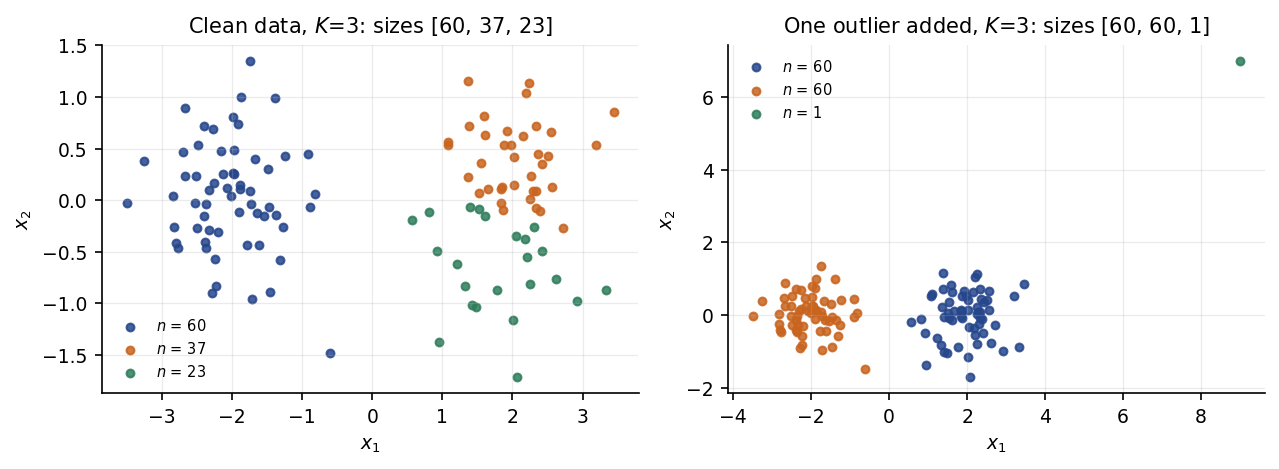
\includegraphics[width=0.92\textwidth,height=0.46\textheight,keepaspectratio]{ch12_x_outlier.png}
  \end{center}
  \begin{mistake}
    Left: two real groups of $60$; forced to $K=3$, $K$-means splits the right-hand group
    into $37+23$. Right: one point added at $(9,7)$ takes a whole cluster to itself, sizes
    $(60,60,1)$. The squared distance in the objective makes one far point worth hundreds
    of ordinary ones. Screen for outliers \emph{before} clustering, and treat a
    near-singleton cluster as a data-quality alarm rather than a discovery.
  \end{mistake}
\end{frame}

\begin{frame}{These methods always return clusters}
  \footnotesize
  \begin{center}
    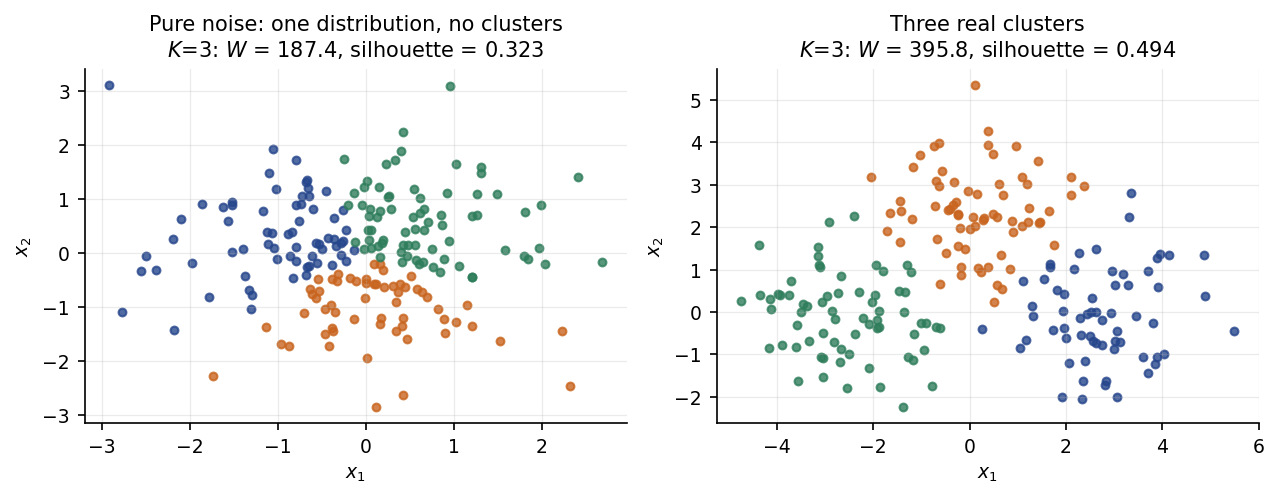
\includegraphics[width=0.92\textwidth,height=0.42\textheight,keepaspectratio]{ch12_noise_clusters.png}
  \end{center}
  \begin{mistake}[{{The error this chapter exists to prevent}}]
    Left panel is $200$ draws from a \emph{single} two-dimensional Gaussian --- there are no
    clusters. $K$-means at $K=3$ returns three tidy, contiguous, roughly equal groups
    ($67,59,74$), cuts the within-cluster sum of squares from $398.0$ to $187.4$
    ($53\%$ ``explained''), and scores a silhouette of $0.323$ --- against $0.494$ for the
    three genuinely separated clusters on the right. There is no threshold on any of these
    numbers that separates the two panels reliably.
  \end{mistake}
\end{frame}

\begin{frame}{How to report a clustering honestly}
  \scriptsize
  \begin{readme}[{{The paragraph that should accompany every segmentation}}]
    \begin{itemize}
      \item \textbf{Say what was done:} features, scaling, dissimilarity, algorithm, $K$,
            \texttt{n\_init}, seed, achieved objective.
      \item \textbf{Say how stable it is:} re-fit on bootstrap samples or random halves and
            report the agreement (ARI, or the share of pairs that stay together).
      \item \textbf{Show the profiles} in original units, so a domain expert can judge
            whether the groups are recognisable.
      \item \textbf{Show one alternative} --- a different $K$ or linkage --- and
            \textbf{call the result a hypothesis}, naming the experiment or downstream
            metric that would confirm it.
    \end{itemize}
  \end{readme}
  \begin{numexample}[{{Measuring stability on this chapter's example}}]
    Re-fit $K=3$ $K$-means on $200$ bootstrap resamples of the $50$ states and compare each
    fit's assignment of all $50$ states with the full-data fit: mean adjusted Rand index
    $\mathbf{0.68}$ (median $0.77$). Reproducible enough to report --- and far from the
    $1.0$ that ``three types of state'' would imply.
  \end{numexample}
  \begin{takeaway}[{{The wording test}}]
    ``We identified three customer types'' claims a finding you cannot support. ``A
    three-cluster solution on standardised spend and tenure features gives three
    interpretable profiles, stable at ARI $0.68$ across bootstrap re-fits; a
    matched-control campaign will test whether the segments respond differently'' claims
    exactly what you have.
  \end{takeaway}
\end{frame}

\begin{frame}{The bridge to Chapter 13}
  \begin{takeaway}[{{Turning structure into something testable}}]
    The gene data makes the link explicit. Clustering \emph{suggested} that the $40$
    samples fall into two groups. To claim a finding you must name the genes and test them
    --- $1000$ two-sample $t$-tests, one per gene. Then you are squarely in Chapter~13:
    $159$ genes have $p<0.05$ (of which $\sim 50$ are expected by chance alone), while
    $\mathbf{105}$ survive Bonferroni at $0.05/1000$, and $91$ of the $100$ smallest
    $p$-values fall in genes $501$--$1000$ --- exactly the block that was constructed to
    differ.
  \end{takeaway}
  \begin{mistake}
    Testing the genes that \emph{defined} the clusters and reporting the $p$-values as if
    the groups had been given in advance. The clustering already used those genes; this is
    post-selection inference, and the $p$-values are optimistic even after Bonferroni.
    An honest version needs an independent sample --- or the selective-inference machinery
    of Chapter~13's appendix.
  \end{mistake}
\end{frame}

% ------------------------------------------------------------
\begin{frame}{Extended Exercise 12.2 --- Clustering pure noise [Python]}
\begin{longexercise}
  Show that the standard diagnostics cannot detect the absence of clusters.
  \begin{enumerate}
    \item Simulate $n=200$ points from a single standard bivariate normal with
          \texttt{rng = np.random.default\_rng(2024)}, and a second data set of three
          genuinely separated clusters (means $(-2.5,0)$, $(2.5,0)$, $(0,2.5)$, unit
          variance).
    \item For $K=1,\dots,8$ record $W(K)$ and, for $K\ge2$, the mean silhouette width on
          both data sets.
    \item Report $W(3)/W(1)$ and the silhouette at $K=3$ for each, and state at which $K$
          the silhouette peaks on the noise.
    \item Propose a diagnostic that \emph{would} have flagged the noise, and say what it
          costs.
  \end{enumerate}
\end{longexercise}
\begin{labnote}[{{Run this live}}]
  The worked solution sits in \texttt{chapter\_12\_lab.ipynb} under
  \emph{Lecture exercises --- worked Python solutions}: the cell headed
  \emph{Extended Exercise 12.2 --- Clustering pure noise [Python]}.
\end{labnote}
\end{frame}

\begin{frame}[fragile]{Solution --- Extended Exercise 12.2 (1/2)}
\begin{solutionbox}[{{Solution --- code}}]
\begin{lstlisting}[basicstyle=\ttfamily\scriptsize]
from sklearn.cluster import KMeans
from sklearn.metrics import silhouette_score

rng   = np.random.default_rng(2024)         # same seed as the slide figure
noise = rng.normal(size=(200, 2))           # ONE Gaussian: no clusters at all
mu    = np.array([[-2.5, 0.], [2.5, 0.], [0., 2.5]])
lab   = rng.integers(0, 3, 200)             # true group of each point
real  = mu[lab] + rng.normal(size=(200, 2))    # three separated clusters
km    = lambda X, K: KMeans(n_clusters=K, n_init=50, random_state=0).fit(X)

for name, X in [('noise', noise), ('real ', real)]:
    W    = {K: km(X, K).inertia_ for K in range(1, 9)}
    sil  = {K: silhouette_score(X, km(X, K).labels_) for K in range(2, 9)}
    peak = max(sil, key=sil.get)            # K with the best silhouette
    print(f'{name} W(3)/W(1)={W[3]/W[1]:.3f} sil(3)={sil[3]:.3f} '
          f'peak K={peak} ({sil[peak]:.3f})')
\end{lstlisting}
\end{solutionbox}
\end{frame}

\begin{frame}{Solution --- Extended Exercise 12.2 (2/2)}
  \scriptsize
\begin{solutionbox}[{{Solution --- output and what it means}}]
  \textbf{Printout.}
  \begin{center}\ttfamily\footnotesize
  noise W(3)/W(1)=0.471 sil(3)=0.323 peak K=8 (0.337)\\[2pt]
  real\ \ W(3)/W(1)=0.248 sil(3)=0.494 peak K=3 (0.494)
  \end{center}
  \begin{itemize}
    \item \textbf{Parts 2--3.} Three clusters of nothing still cut the objective by
          $52.9\%$ ($398.0\to187.4$) and score a silhouette of $0.323$, a value many
          practitioners would call ``reasonable structure''. On the noise the silhouette
          \emph{rises} again to $0.337$ at $K=8$: it never says ``stop''. Only the
          comparison with the real data ($0.494$, peaking exactly at $K=3$) exposes it ---
          and in an application there is no real data to compare with.
    \item \textbf{Part 4 --- a diagnostic that works.} Compare the observed $\log W(K)$ with
          its distribution under a simulated \emph{no-cluster} reference: the gap statistic.
          Cost: you must specify the null, it is far more computation, and it has power only
          for well-separated clusters. There is no free validation here.
  \end{itemize}
  \smallskip
  \textit{Common mistake:} quoting ``$K=3$ explains $53\%$ of the variation'' as evidence
  of three groups. On this noise it is literally true and completely empty.
\end{solutionbox}
\end{frame}

% ============================================================
\section{Python Lab}
% ============================================================

\begin{frame}{Python lab --- run it live in the notebook}
  \begin{labnote}[{{Companion notebook: \texttt{chapter\_12\_lab.ipynb}}}]
    The code in this section is meant to be \textbf{demonstrated live}. Open the companion
    Jupyter notebook and run it cell by cell:
    \begin{itemize}
      \item \S1, \emph{PCA on USArrests} --- loadings, scores, PVE, the biplot and the
            scree plot, and the scaled-vs-unscaled comparison;
      \item \S2, \emph{K-means} --- $K=2,3,4$, cluster profiles in original units, and the
            local-optimum experiment;
      \item \S3, \emph{Hierarchical clustering} --- four linkages, cutting the tree, and
            how much the partition moves;
      \item \S4, \emph{High-dimensional data} --- PCA and clustering on the bundled
            gene-expression data (with the optional \texttt{NCI60} branch);
      \item \S5, \emph{Practical issues} --- outliers, and clustering pure noise.
    \end{itemize}
    Data loads via the \texttt{ISLP} package or the bundled CSV files; \S6,
    \emph{Exercises} ends the notebook with hands-on tasks, after the worked solutions to
    every \texttt{[Python]} exercise in this deck.
  \end{labnote}
\end{frame}

\begin{frame}[fragile]{PCA in scikit-learn}
  \begin{lstlisting}
import numpy as np, pandas as pd                     # arrays and frames
from sklearn.decomposition import PCA                # PCA
from sklearn.preprocessing import StandardScaler     # z-scoring

USA = load('USArrests', index_col=0)                 # 50 states x 4 features
Xs  = StandardScaler().fit_transform(USA)            # ALWAYS decide this on purpose
pca = PCA().fit(Xs)                                  # all min(n-1, p) components

print(np.round(pca.explained_variance_ratio_, 4))    # [0.6201 0.2474 0.0891 0.0434]
print(np.round(np.cumsum(pca.explained_variance_ratio_), 4))   # cumulative PVE
loadings = pd.DataFrame(pca.components_.T, index=USA.columns,
                        columns=[f'PC{i+1}' for i in range(4)])
print(loadings.round(3))                             # signs may be flipped: fine
Z = pca.transform(Xs)                                # the scores, n x p
  \end{lstlisting}
\end{frame}

\begin{frame}[fragile]{$K$-means, and proving the local-optimum problem}
  \begin{lstlisting}
from sklearn.cluster import KMeans                    # Lloyd's algorithm

km = KMeans(n_clusters=3, n_init=50, random_state=0).fit(Xs)   # 50 restarts
print(round(km.inertia_, 3))                          # 79.922 (sum of sq. dists)
print(USA.assign(cluster=km.labels_)                  # profiles in RAW units
         .groupby('cluster').mean().round(1))

w = [KMeans(n_clusters=4, n_init=1, random_state=s).fit(Xs).inertia_
     for s in range(20)]                              # twenty single-start runs
print(np.round(sorted(w), 3))                         # 57.554 ... 77.856
print('distinct local optima:', len(set(np.round(w, 3))))       # 9
  \end{lstlisting}
\end{frame}

\begin{frame}[fragile]{Hierarchical clustering with scipy}
  \begin{lstlisting}
from scipy.cluster.hierarchy import linkage, dendrogram, fcluster
from scipy.spatial.distance import squareform

for method in ['complete', 'average', 'single', 'centroid']:
    Zl = linkage(Xs, method=method)                   # Euclidean by default
    lab = fcluster(Zl, 3, criterion='maxclust')       # cut into 3 clusters
    print(f'{method:9s} sizes {np.bincount(lab)[1:]}  top fusion {Zl[-1,2]:.2f}')

Dcorr = 1 - np.corrcoef(Xs)                           # correlation-based distance
Zc = linkage(squareform(Dcorr, checks=False), 'complete')   # needs condensed form
dendrogram(Zl, labels=USA.index.tolist(), leaf_font_size=6) # HEIGHT is the message
  \end{lstlisting}
\end{frame}

% ============================================================
\section{Summary}
% ============================================================

\begin{frame}{Chapter 12 in one slide}
  \begin{block}{What we accomplished}
    Finding structure in $X$ alone --- and reporting it honestly, without a test error to
    hide behind.
  \end{block}
  \begin{itemize}
    \item Why unsupervised learning has no validation, and what can be borrowed instead:
          stability, interpretability, a downstream supervised task.
    \item PCA: loadings, scores, orthogonality, PVE, the scree plot, the biplot, sign
          indeterminacy, and the fact that scaling changes everything.
    \item $K$-means: the within-cluster objective, Lloyd's algorithm, local optima
          measured rather than asserted, and \texttt{n\_init}.
    \item Hierarchical clustering: the dendrogram, height versus horizontal position,
          four linkages, and the dissimilarity measure.
    \item Practice: outliers, clusters in pure noise, and the wording of an honest report.
  \end{itemize}
\end{frame}

\begin{frame}{Key formulas at a glance (1/2)}
  \footnotesize
  \begin{description}
    \item[Standardising] $\tilde x_{ij}=(x_{ij}-\bar x_j)/s_j$; PCA on standardised data
          $=$ PCA on the correlation matrix.
    \item[First component] $\max_{\phi_1}\frac1n\sum_i\bigl(\sum_j\phi_{j1}x_{ij}\bigr)^2$
          s.t.\ $\sum_j\phi_{j1}^2=1$; solution $=$ top eigenvector of the covariance
          (or correlation) matrix.
    \item[Scores] $z_{im}=\sum_{j=1}^{p}\phi_{jm}x_{ij}$, with $x$ centred.
    \item[Orthogonality] $\phi_m^\top\phi_{m'}=0$ and $\mathrm{Cov}(z_{\cdot m},z_{\cdot m'})=0$
          for $m\ne m'$.
    \item[Variance partition] $\lambda_m=\mathrm{Var}(z_{\cdot m})$ and
          $\sum_{m=1}^{p}\lambda_m=\sum_{j=1}^{p}\mathrm{Var}(X_j)$ \ ($=p$ if standardised).
    \item[PVE] $\mathrm{PVE}_m=\lambda_m/\sum_{m'}\lambda_{m'}
          =\sum_i z_{im}^2\big/\sum_j\sum_i x_{ij}^2$; \ cumulative
          $\sum_{m\le M}\mathrm{PVE}_m$.
    \item[Sign indeterminacy] $\phi_m\mapsto-\phi_m$, $z_{im}\mapsto-z_{im}$, $\lambda_m$
          unchanged.
    \item[Low-rank view] $\min_{a,b}\sum_{ij}\bigl(x_{ij}-\sum_{m\le M}a_{im}b_{jm}\bigr)^2$
          is solved by $a_{im}=z_{im}$, $b_{jm}=\phi_{jm}$; residual SS
          $=n\sum_{m>M}\lambda_m$.
    \item[Two-variable case] $\mathbf{R}=\bigl(\begin{smallmatrix}1&r\\r&1\end{smallmatrix}\bigr)
          \Rightarrow \lambda_{1,2}=1\pm r$, $\phi_{1,2}=\tfrac{1}{\sqrt2}(1,\pm1)^\top$,
          $\mathrm{PVE}_1=(1+r)/2$.
  \end{description}
\end{frame}

\begin{frame}{Key formulas at a glance (2/2)}
  \footnotesize
  \begin{description}
    \item[$K$-means objective] $\min_{C_1..C_K}\sum_{k}W(C_k)$ with
          $W(C_k)=\frac{1}{|C_k|}\sum_{i,i'\in C_k}\sum_j (x_{ij}-x_{i'j})^2$.
    \item[Centroid form] $W(C_k)=2\sum_{i\in C_k}\sum_j (x_{ij}-\bar x_{kj})^2$, \
          $\bar x_{kj}=\frac{1}{|C_k|}\sum_{i\in C_k}x_{ij}$ \ (software reports the
          version without the $2$).
    \item[Assignment step] $i \mapsto \arg\min_k \|x_i-\bar x_k\|^2$; the mean minimises
          $\sum_{i\in C_k}\|x_i-c\|^2$, which is why both steps decrease $W$.
    \item[SS decomposition] $\mathrm{TSS}=\sum_i\sum_j(x_{ij}-\bar x_j)^2 = W + \mathrm{BSS}$;
          ``variance explained'' $=1-W/\mathrm{TSS}$ (rises with $K$ by construction).
    \item[Euclidean dissimilarity] $d(i,i')=\sum_{j}(x_{ij}-x_{i'j})^2$.
    \item[Correlation dissimilarity] $d(i,i')=1-r_{ii'}$, $r_{ii'}$ the correlation of the
          two feature profiles ($p\ge3$).
    \item[Linkage] complete $\max_{i\in A,i'\in B}d(i,i')$; \ single $\min$; \
          average $\frac{1}{|A||B|}\sum\sum d(i,i')$; \ centroid $\|\bar x_A-\bar x_B\|^2$.
    \item[Silhouette] $s_i=\dfrac{b_i-a_i}{\max(a_i,b_i)}\in[-1,1]$, with $a_i$ the mean
          distance to $i$'s own cluster and $b_i$ the smallest mean distance to another
          cluster.
    \item[Agreement of two partitions] adjusted Rand index: $0$ for chance agreement, $1$
          for identical partitions.
  \end{description}
\end{frame}

\begin{frame}{Vocabulary checklist}
  \footnotesize
  \begin{tabular}{@{}ll@{}}
    \toprule
    \textbf{Term} & \textbf{Meaning} \\
    \midrule
    Loading $\phi_{jm}$ & weight of feature $j$ in component $m$; defines a direction \\
    Score $z_{im}$ & coordinate of observation $i$ along component $m$ \\
    PVE & share of total variance carried by a component \\
    Scree plot & PVE against component number; the ``elbow'' is a heuristic \\
    Biplot & scores and loading arrows in one picture \\
    Sign indeterminacy & $\phi_m$ and $-\phi_m$ are the same component \\
    Within-cluster variation $W$ & the $K$-means objective; \texttt{inertia\_} \\
    Local optimum & a partition no single move improves; not necessarily the best \\
    \texttt{n\_init} & number of random starts kept for the best objective \\
    Dendrogram & tree of fusions; \emph{height} carries the information \\
    Linkage & rule for the dissimilarity between two clusters \\
    Chaining & single linkage's habit of growing one long cluster \\
    Inversion & a fusion drawn below one of its children (centroid linkage) \\
    Silhouette width & how much better an observation fits its own cluster \\
    Gap statistic & compares $W(K)$ with a no-cluster reference distribution \\
    \bottomrule
  \end{tabular}
\end{frame}

\begin{frame}{Decision rules of thumb}
  \begin{itemize}
    \item Features in different units $\Rightarrow$ \textbf{standardise}, and say so.
          \texttt{USArrests} unscaled gives PC1 $=$ Assault at $96.6\%$.
    \item Want a picture of $p$ variables $\Rightarrow$ PCA, report cumulative PVE, and
          admit what the projection discards.
    \item Choosing $M$ or $K$ $\Rightarrow$ heuristics propose, the domain decides. Never
          call an elbow a result.
    \item Running $K$-means $\Rightarrow$ \texttt{n\_init} $\ge 20$, fixed seed, report the
          objective.
    \item $n$ small enough for an $n\times n$ matrix and no idea what $K$ is
          $\Rightarrow$ hierarchical; then justify linkage \emph{and} dissimilarity.
    \item Profiles matter more than levels $\Rightarrow$ correlation-based dissimilarity;
          levels matter $\Rightarrow$ Euclidean.
    \item Before believing any partition $\Rightarrow$ re-fit on halves or bootstraps and
          report the agreement.
    \item Writing it up $\Rightarrow$ ``hypothesis'', plus the experiment that would test
          it.
  \end{itemize}
\end{frame}

\begin{frame}{Common pitfalls}
  \begin{alertblock}{Don't}
    \begin{enumerate}
      \item Run PCA on unstandardised variables in different units and celebrate a huge
            PVE.
      \item Assume your figure is wrong because a component's sign differs from the book's.
      \item Read horizontal proximity in a dendrogram as similarity.
      \item Run $K$-means once and report the partition as \emph{the} partition.
      \item Compare $W$ across different $K$ and call the decrease ``validation''.
      \item Cluster with outliers still in, then report the singleton cluster as a segment.
      \item Present clusters found in a single unimodal cloud as customer types.
      \item Test the very features that defined the clusters and quote the $p$-values
            as if the groups were given in advance.
    \end{enumerate}
  \end{alertblock}
\end{frame}

\begin{frame}{Self-check questions}
  \scriptsize
  \begin{readme}[{{Quick self-assessment}}]
    \begin{enumerate}
      \item Why can a held-out sample not validate a clustering?
      \item What are the two constraints defining the second principal component?
      \item \texttt{USArrests} unscaled gives $\mathrm{PVE}_1=96.6\%$; scaled it gives
            $62.0\%$. Which do you report, and why?
      \item Your PC2 loadings are exactly the negatives of a colleague's. Who is wrong?
      \item Two runs of $K$-means at $K=4$ give $W=57.554$ and $W=58.242$. What do you do?
      \item Complete linkage cut at $3$ gives $(31,11,8)$; single linkage gives
            $(48,1,1)$. Which is correct?
      \item Pure noise gives a silhouette of $0.323$ at $K=3$. What follows?
    \end{enumerate}
  \end{readme}
  \begin{takeaway}[{{Answers}}]
    (1) Assigning a held-out point to its nearest centroid \emph{defines} its label, so the
    ``error'' is zero by construction. (2) Unit norm and orthogonality to $\phi_1$.
    (3) The scaled one --- otherwise you are reporting units. (4) Neither: signs are
    arbitrary. (5) Keep $W=57.554$ and raise \texttt{n\_init}; the other run is simply
    worse. (6) Both, for their own assumption about cluster shape --- the question is which
    assumption you can defend. (7) That the silhouette cannot detect the absence of
    clusters, so it must not be used as evidence that clusters exist.
  \end{takeaway}
\end{frame}

\begin{frame}{Five things to remember}
  \begin{takeaway}[{{Chapter 12 in five lines}}]
    \begin{enumerate}
      \item \textbf{No response means no test error.} Every answer here is a hypothesis;
            nothing in the data can call it wrong.
      \item \textbf{Scaling is a decision, not a formality.} On \texttt{USArrests} it moves
            $\mathrm{PVE}_1$ from $62.0\%$ to $96.6\%$ and turns PC1 into one variable.
      \item \textbf{$K$-means finds a local optimum.} Twenty single starts at $K=4$ gave
            nine different answers, the worst $35\%$ off; \texttt{n\_init} is not optional.
      \item \textbf{In a dendrogram, only height means anything} --- and the linkage and the
            distance can matter more than the algorithm.
      \item \textbf{These methods always return clusters}, including from pure noise. Report
            the choices, the stability, and the test you would run next.
    \end{enumerate}
  \end{takeaway}
\end{frame}

% ============================================================
\appendix
\AtBeginSection[]{}
\section{Appendix: optional and advanced material}
% ============================================================

\begin{frame}{Appendix --- what is in here, and why}
  \small
  Nothing in the appendix is needed to follow the chapter: each slide is a
  formal derivation, a longer worked exercise, or a side topic. Read it when
  you want the full story, or when a later chapter sends you back here.
  \begin{block}{Contents of the appendix}
    \begin{itemize}
      \item \textbf{The two forms of the $K$-means objective} --- the algebraic identity
            that turns the all-pairs definition into the centroid form. Quoted as a fact in
            the main deck because the algebra is a distraction there.
      \item \textbf{PCA as the best low-rank approximation} --- why maximising variance and
            minimising reconstruction error are the same problem, and the residual formula.
      \item \textbf{PCA with missing values} --- the matrix-completion algorithm, needed in
            practice and beyond the exam.
      \item \textbf{The silhouette width} --- the formula, and what it looks like on
            \texttt{USArrests}.
      \item \textbf{Extended Exercise 12.3} --- a full clustering workflow on the bundled
            gene-expression data. It needs $20$ minutes of lab time, so a 180-minute
            session may not reach it.
    \end{itemize}
  \end{block}
\end{frame}

\begin{frame}{Derivation: the two forms of the $K$-means objective}
  \footnotesize
  \begin{block}{Claim}
    $\displaystyle \frac{1}{|C_k|}\sum_{i,i'\in C_k}\sum_{j=1}^{p}(x_{ij}-x_{i'j})^{2}
     = 2\sum_{i\in C_k}\sum_{j=1}^{p}(x_{ij}-\bar x_{kj})^{2}$.
  \end{block}
  \scriptsize
  Fix a feature $j$, write $n_k=|C_k|$ and $\bar x=\bar x_{kj}$. Expand around the mean:
  \[
    \sum_{i,i'\in C_k}(x_{ij}-x_{i'j})^{2}
    = \sum_{i,i'}\bigl[(x_{ij}-\bar x)-(x_{i'j}-\bar x)\bigr]^{2}
    = \sum_{i,i'}\Bigl[(x_{ij}-\bar x)^2 + (x_{i'j}-\bar x)^2
      - 2(x_{ij}-\bar x)(x_{i'j}-\bar x)\Bigr].
  \]
  The first two double sums each give $n_k\sum_{i}(x_{ij}-\bar x)^2$; the cross term
  factorises into $-2\bigl(\sum_i (x_{ij}-\bar x)\bigr)^2$, which is \textbf{zero} because
  deviations from the mean sum to zero. Hence
  $\sum_{i,i'\in C_k}(x_{ij}-x_{i'j})^{2}=2n_k\sum_{i\in C_k}(x_{ij}-\bar x_{kj})^{2}$,
  and dividing by $n_k$ and summing over $j$ gives the claim.
  \begin{takeaway}
    Two consequences: the objective depends on the data only through squared Euclidean
    distances, and the centroid form shows why re-computing means can never increase $W$
    --- the mean is the minimiser of $\sum_i \|x_i - c\|^2$.
  \end{takeaway}
\end{frame}

\begin{frame}{PCA as the best low-rank approximation}
  \footnotesize
  \begin{block}{Eckart--Young, in the notation of this chapter}
    For any $M\le \min(n-1,p)$,
    \[
      \min_{A\in\mathbb{R}^{n\times M},\,B\in\mathbb{R}^{p\times M}}
      \ \sum_{i=1}^{n}\sum_{j=1}^{p}\Bigl(x_{ij}-\sum_{m=1}^{M}a_{im}b_{jm}\Bigr)^{2}
      \ =\ n\sum_{m=M+1}^{p}\lambda_m ,
    \]
    attained at $a_{im}=z_{im}$, $b_{jm}=\phi_{jm}$ (unique up to rotation within the
    retained subspace, and up to the sign of each component).
  \end{block}
  \begin{readme}
    \begin{itemize}
      \item Total sum of squares is $n\sum_m \lambda_m$; the first $M$ components account
            for $n\sum_{m\le M}\lambda_m$, so the leftover is the tail of the eigenvalues.
      \item Dividing through, the \emph{fraction} of squared error left after $M$
            components is exactly $1-\sum_{m\le M}\mathrm{PVE}_m$. For
            \texttt{USArrests} at $M=2$ that is $13.2\%$.
      \item ``Rotation within the subspace'' is why factor analysis can rotate loadings
            (varimax) without changing the fit: the \emph{subspace} is identified, the axes
            inside it only by the variance-ordering convention.
    \end{itemize}
  \end{readme}
\end{frame}

\begin{frame}{PCA with missing values: matrix completion}
  \footnotesize
  \begin{block}{Algorithm (hard-impute)}
    \begin{enumerate}
      \item Fill each missing $x_{ij}$ with the column mean $\bar x_j$ of the observed
            entries.
      \item Compute the rank-$M$ PCA approximation
            $\hat x_{ij}=\sum_{m\le M} z_{im}\phi_{jm}$ of the completed matrix.
      \item Replace \emph{only the missing} entries by their $\hat x_{ij}$; keep observed
            entries as they are.
      \item Repeat 2--3 until the fitted values stop changing.
    \end{enumerate}
  \end{block}
  \begin{readme}
    Each iteration solves the low-rank problem of the previous slide over the observed
    entries only, so the objective decreases monotonically --- the same
    ``guaranteed to converge, not guaranteed to be optimal'' situation as $K$-means.
    $M$ must be chosen, and the method assumes entries are missing for reasons unrelated to
    their values.
  \end{readme}
  \begin{industry}[{{Recommenders: the same algorithm under another name}}]
    A user-by-item rating matrix is mostly missing. Low-rank completion of it is the
    classical collaborative-filtering engine --- $M$ latent factors standing in for taste.
  \end{industry}
\end{frame}

\begin{frame}{The silhouette width}
  \scriptsize
  \begin{block}{Definition}
    For observation $i$ in cluster $C_k$, let $a_i$ be its mean distance to the other
    members of $C_k$ and $b_i=\min_{k'\ne k}$ (mean distance to members of $C_{k'}$). Then
    \[
      s_i=\frac{b_i-a_i}{\max(a_i,b_i)}\in[-1,1] .
    \]
  \end{block}
  \begin{center}
    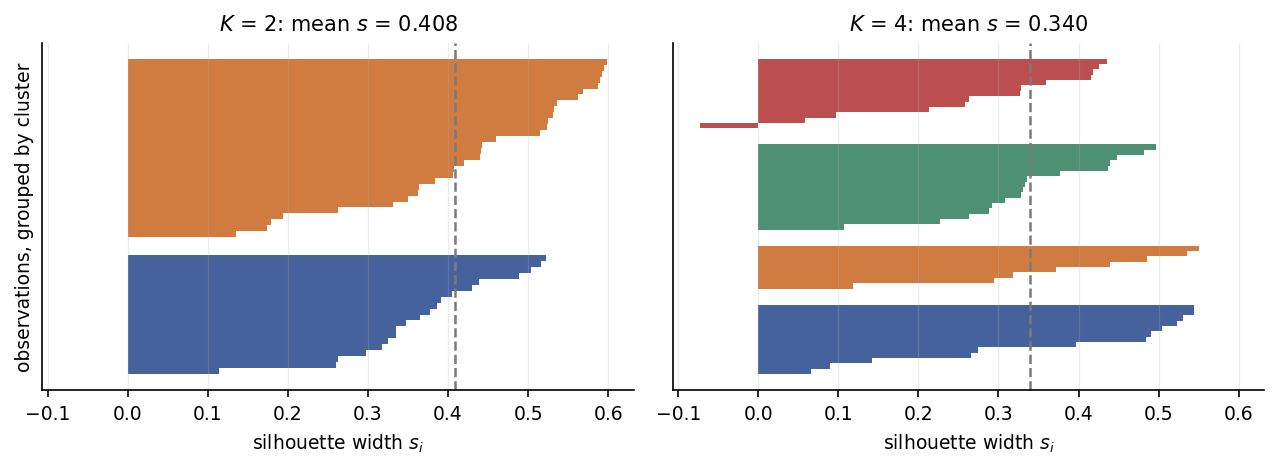
\includegraphics[width=0.86\textwidth,height=0.34\textheight,keepaspectratio]{ch12_x_silhouette.png}
  \end{center}
  \begin{takeaway}
    On standardised \texttt{USArrests} the mean silhouette is $0.408$ at $K=2$ and $0.340$
    at $K=4$, so the criterion prefers $K=2$. Negative $s_i$ marks observations that sit
    closer to another cluster than their own. Useful for \emph{ranking} candidate $K$;
    useless for deciding whether any clustering is real (see the noise example).
  \end{takeaway}
\end{frame}

\begin{frame}{Extended Exercise 12.3 --- A full workflow on gene expression [Python]}
  \footnotesize
\begin{longexercise}
  \texttt{Ch12Ex13.csv} holds $1000$ genes (rows) measured on $40$ tissue samples
  (columns); the first $20$ samples are healthy and the last $20$ diseased --- a label you
  may use \emph{only} to score your answer at the end, never to fit.
  \begin{enumerate}
    \item Cluster the $40$ \emph{samples} with complete, average and single linkage under
          (i) Euclidean distance and (ii) correlation-based distance $1-r$. Cut each tree
          into two clusters.
    \item Score all six partitions against the true labels with the adjusted Rand index.
          Which decision --- linkage or dissimilarity --- mattered more?
    \item Run PCA on the samples. What does PC1 do, and how much variance does it explain?
    \item Which genes differ between the groups? Rank them and count how many survive a
          Bonferroni threshold at $0.05/1000$.
  \end{enumerate}
\end{longexercise}
\begin{labnote}[{{Run this live}}]
  The worked solution sits in \texttt{chapter\_12\_lab.ipynb} under
  \emph{Lecture exercises --- worked Python solutions}: the cell headed
  \emph{Extended Exercise 12.3 --- A full workflow on gene expression [Python]}.
\end{labnote}
\end{frame}

\begin{frame}[fragile]{Solution --- Extended Exercise 12.3 (1/3)}
\begin{solutionbox}[{{Solution --- code: clustering under two dissimilarities}}]
\begin{lstlisting}[basicstyle=\ttfamily\scriptsize]
import numpy as np
from scipy.cluster.hierarchy import linkage, fcluster
from scipy.spatial.distance import squareform
from sklearn.metrics import adjusted_rand_score

G = load('Ch12Ex13', header=None).values   # 1000 genes x 40 samples
X = G.T                                    # cluster the SAMPLES: 40 x 1000
truth = np.array([0]*20 + [1]*20)          # for SCORING only, never for fitting

for nm, arg in [('eucl', X), ('1-r', squareform(1-np.corrcoef(X), checks=False))]:
    for m in ('complete', 'average', 'single'):
        lab = fcluster(linkage(arg, method=m), 2, criterion='maxclust')
        print(nm, m, np.bincount(lab)[1:], round(adjusted_rand_score(truth, lab), 3))
\end{lstlisting}
\end{solutionbox}
\end{frame}

\begin{frame}[fragile]{Solution --- Extended Exercise 12.3 (2/3)}
  \footnotesize
\begin{solutionbox}[{{Solution --- code: PCA and the per-gene tests, and the printout}}]
\begin{lstlisting}[basicstyle=\ttfamily\scriptsize]
from scipy import stats
from sklearn.decomposition import PCA

p = PCA().fit(X - X.mean(0)); Z = p.transform(X - X.mean(0))   # PCA on the samples
print('PVE1', round(p.explained_variance_ratio_[0], 3),
      ' PC1 group means', round(Z[:20, 0].mean(), 2), round(Z[20:, 0].mean(), 2))
t, pv = stats.ttest_ind(G[:, 20:], G[:, :20], axis=1)   # 1000 two-sample t-tests
print((pv < 0.05).sum(), (pv < 0.05/1000).sum())        # nominal, then Bonferroni
\end{lstlisting}
  \begin{center}\ttfamily\scriptsize
  eucl complete [20 20] 1.0\qquad 1-r complete [30 10] 0.235\\
  eucl average\ \ [20 20] 1.0\qquad 1-r average\ \ [31\ \ 9] 0.188\\
  eucl single\ \ \ [20 20] 1.0\qquad 1-r single\ \ \ [39\ \ 1] 0.0\\[2pt]
  PVE1 0.127\ \ PC1 group means -11.75 11.75\qquad 159 105
  \end{center}
\end{solutionbox}
\end{frame}

\begin{frame}{Solution --- Extended Exercise 12.3 (3/3)}
  \footnotesize
\begin{solutionbox}[{{Solution --- interpretation}}]
  \begin{itemize}
    \item \textbf{Parts 1--2.} Euclidean distance recovers the truth under all three
          linkages; $1-r$ under none. The \textbf{dissimilarity} mattered enormously, the
          linkage barely at all: the diseased group differs by a \emph{level shift} in genes
          $501$--$1000$ (mean absolute difference $0.61$ there versus $0.30$ elsewhere), and
          $1-r$ is engineered to ignore levels.
    \item \textbf{Part 3.} PC1 explains only $12.7\%$ yet separates the groups completely
          (means $-11.75$ vs $+11.75$): with $p\gg n$ a modest PVE can be the whole story.
    \item \textbf{Part 4.} $159$ genes have $p<0.05$, but $\sim 50$ are expected under the
          global null. $\mathbf{105}$ survive Bonferroni at $5\times10^{-5}$, and $91$ of
          the $100$ smallest $p$-values lie in genes $501$--$1000$ --- Chapter~13, and the
          only part of this analysis with a guarantee attached.
  \end{itemize}
\end{solutionbox}
\begin{mistake}
  Using \texttt{truth} anywhere before step 2. If the labels are available you have a
  \emph{supervised} problem; clustering is what you do when they are not.
\end{mistake}
\end{frame}

\end{document}
